\chapter{Návrh ovládacích karet}
\section{Základní požadavky na Ovládací karty}
    Následující seznam popisuje základní požadavky na ovládací karty, seznam je seřazen podle priorit.
    \begin{enumerate}
        \item Schopnost ovládat měřící karty.
        \item Možnost komunikace pomocí 100\,Mbit Ethernetu.
        \item Dostupnost komponentů.
        \item Cena komponentů.
    \end{enumerate}

    \section{Funkční bloky}
    \begin{figure}[ht!]
        \centering
        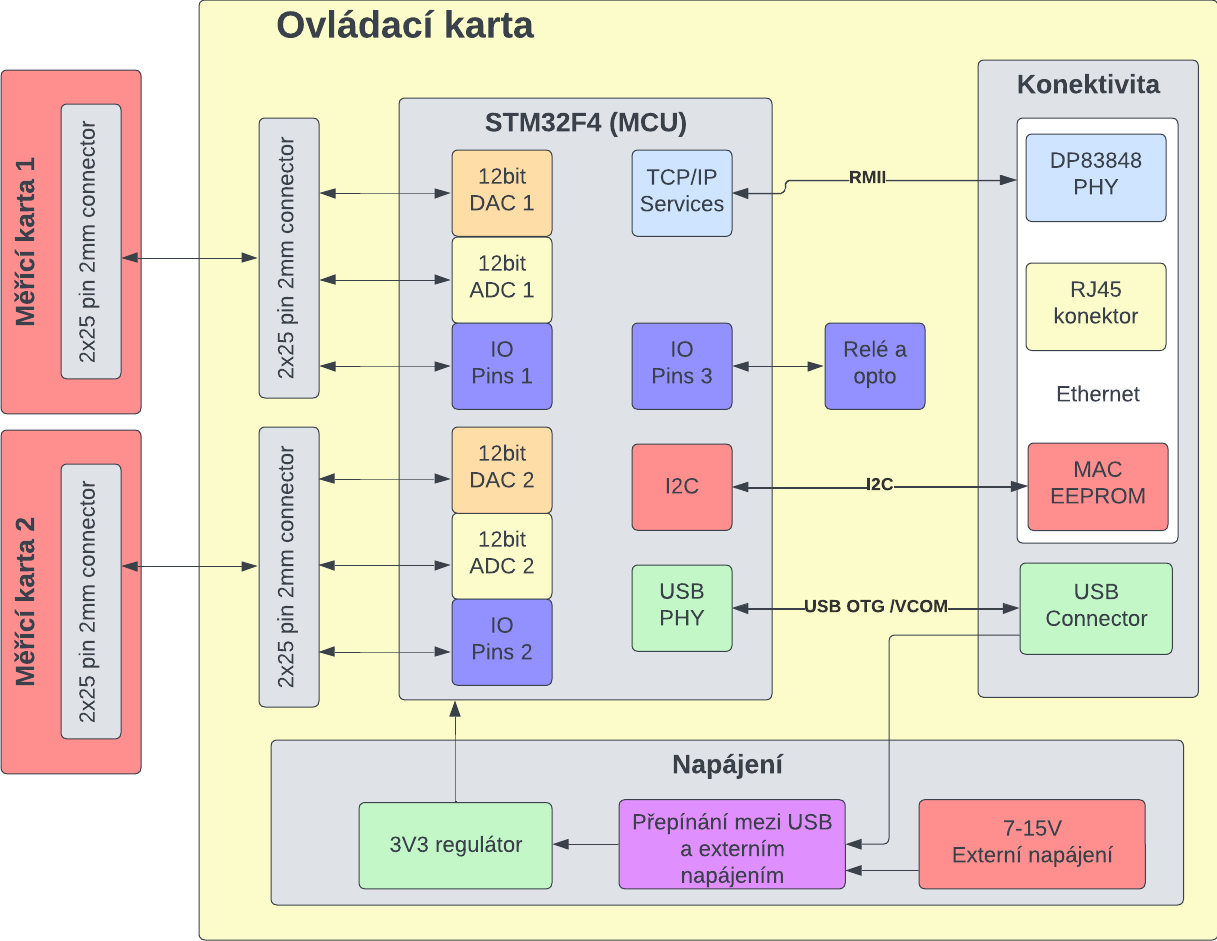
\includegraphics[width = 1\textwidth]{obrazky/ovladaci_karta_diag.png}
        \caption{Funkční diagram ovládací karty}
        \label{fig:Funkční diagram ovládací karty}
        
    \end{figure}

    Ovládací karta obsahuje několik pomyslných funkčních bloků (Obr. \ref{fig:Funkční diagram ovládací karty}).
    Jednotlivé bloky jsou podrobněji popsány v následujících kapitolách. Celé schéma k ovládací kartě je v příloze
    na konci tohoto dokumentu.

    \subsection{Mikrokontrolér a jeho periférie}
    Ovládací karta je založena na 32-bitovém mikrokontroléru STM32F407ZGT6 s Cortex M4 jádrem.
    Tento mikrokontrolér disponuje 114 I/O piny (3V3 logika), dvěma nezávislými 12-bit A/D a D/A převodníky,
    nativní podporou USB OTG a 100\,Mbit Ethernet MAC vrstvou. Právě díky těmto vlastnostem, je tento
    mikrokontrolér vhodný pro ovládání měřících karet a komunikaci s PC.\\

    Pro komunikaci s PC aplikací se primárně počítá s telnet serverem,
    který běží na mikrokontroléru. Nicméně pro debugovací
    účely je možno s ovládací kartou komunikovat i pomocí USB.
    K programování mikrokontroléru lze použít interface SWD, JTAG nebo DFU (USB bootloader).\\

    Jednotlivé shift registry a multiplexery jsou ovládány, skrze ovládací kartu, pomocí metody bit bangingu.
    Dále ovládací karta poskytuje 12-bitový DA a AD převodík.\cite{MARTINT}.\\

    Ovládací karta obsahuje i další periferie jako například CAN, LIN, RTC, opticky oddělené vstupy a výstupy apod.
    Tyto periferie slouží k použití karty v jiném projektu než je právě diplomová práce a proto nejsou podrobněji diskutovány.


    \subsubsection{D/A převodník}
    STM32F407ZGT6 nabízí dva 12-bit D/A převodníky s možností využití integrovaného bufferu v podobě
    invertujícího operačního zesilovače. Nicméně podle datasheetu
    je možné použít výstupní buffer pouze do velikosti kapacitní zátěže 50\,pF.
    Kapacitní zátěž D/A převodníku bude rovna parazitním kapacitám, které nelze jednoznačně určit
    a vstupní kapacitě 80 komparátorů (V+ proti GND). Každý z komparátorů má svou vstupní kapacitu
    přibližně 3\,pF. Dohromady tedy vznikne kapacitní zátěž minimálně 240\,pF.\cite{DAC}\\
    \begin{figure}[ht!]
        \centering
        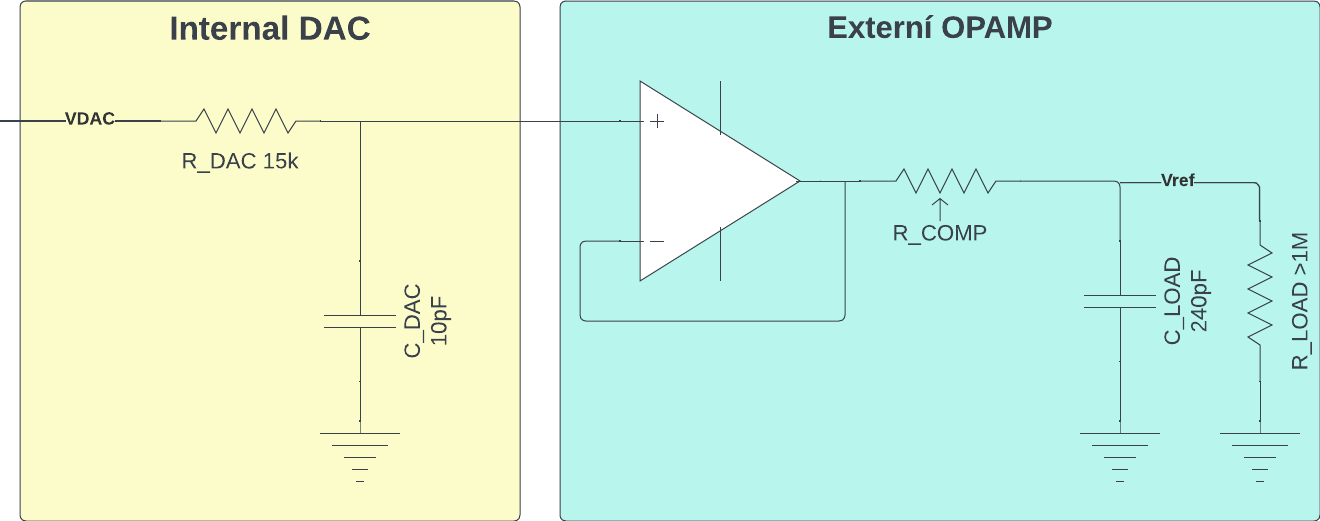
\includegraphics[width = 1\textwidth]{obrazky/DAC_OPAMP.png}
        \caption{DAC-externí zesilovač}
        \label{fig: DAC-externí zesilovač}
        
    \end{figure}

    Pro použití D/A převodníku je použit externí operační zesilovač v zapojení (Obr. \ref{fig: DAC-externí zesilovač}).
    V tomto zapojení je rychlost D/A převodníku limitována kapacitou pinu D/A převodníku C\_DAC (cca 10\,pF)
    a vnitřním odporem R\_DAC (cca 15\,k$\Omega$). Mezní kmitočet nezatíženého D/A převodníku pak lze určit následovně.
    \begin{equation}
        f_{max} = \frac{1}{2\pi \cdot  C_{dac} \cdot  R_{dac}} = \frac{1}{2\pi \cdot 10\,pF \cdot 15\,k\Omega} = 1,06\,MHz
    \end{equation}

    Kapacitní zátěž společně s výstupním odporem operačního zesilovače by mohla
    způsobit nestabilitu a s tím spojené nežádoucí oscilace v časové oblasti.
    Z tohoto důvodu datasheet použitého operačního zesilovače AD8531 doporučuje použít v případě vyšší kapacitní zátěže tzv. snubber network.
    V datasheetu je možno nalézt následující hodnoty součástek pro různou kapacitní zátěž (v Obr. \ref{fig: DAC-externí zesilovač} realizováno
    kombinací součástek C\_SNUBB a R\_COMP).
    \begin{figure}[ht!]
        \centering
        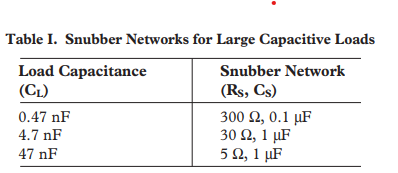
\includegraphics[]{obrazky/snubber_values.png}
        \caption{Snubber Network (obrázek převzat z \cite{OPA_datasheet})}
        \label{fig: Snubber Network}
    \end{figure}

    Protože datasheet neuvádí hodnoty součástek pro kapacitní zátěž 240\,pF, je odpor R\_COMP realizován
    trimmerem pro možnost kalibrace. Hodnota kapacity C\_SNUBB byla zvolena 100\,nF.\\
    Kalibrace je prováděna tak, že se na výstupu D/A převodníku nastaví obdélníkový
    signál o frekvenci 500\,kHz a poté se trimmerem nastaví taková hodnota, aby v časové oblasti
    byl co nejmenší překmit\cite{DAC_stability,OPA_stability}.\\

    \subsubsection{Programování a debuging}
    Pro účely debugování a programování mikrokontroléru jsou zpřístupněny SWD a JTAG piny.
    Dále je možno modifikovat konfiguraci mikrokontroléru pomocí jumperů, které jsou propojeny
    s boot piny mikrokontroléru. Při normálním provozu se počítá s programováním pomocí SWD rozhraní.
    Případně je také možné mikrokontrolér naprogramovat přes USB konektor pomocí zabudovaného DFU.

    \subsubsection{Konfigurace hodinového signálu}
    
    Mikrokontrolér má vysokou variabilitu v konfiguraci hodinových signálů.
    K požadovaným funkcím ovládací karty je vhodné použít externí krystalový rezonátor, který bude
    připojen do High Speed Clock pinů mikrokontroléru. V případě ovládací karty bylo použit 8\,MHz
    krystalového rezonátoru ABM3B-8.000MHZ-D2-T společně s 2x27\,pF zatěžovacími kapacitory.\\

    %%\begin{figure}[ht!]
    %%    \centering
    %%    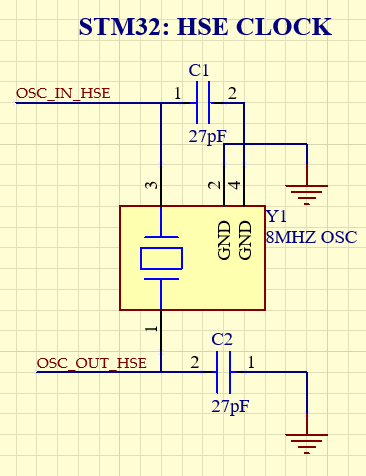
\includegraphics[height = 0.2\textheight]{obrazky/CLK_rezonator.png}
    %%    \caption{8\,MHz krystalový rezonátor}
    %%    \label{fig: MHz krystalový rezonátor}
    %%\end{figure}

    Pro jednodušší konfiguraci hodinových signálů mikrokontroléru bylo využito programu STM32CubeMX.
    Výsledná konfigurace hodinových signálů je znázorněna na následujícím obrázku.

    \begin{figure}[ht!]
        \centering
        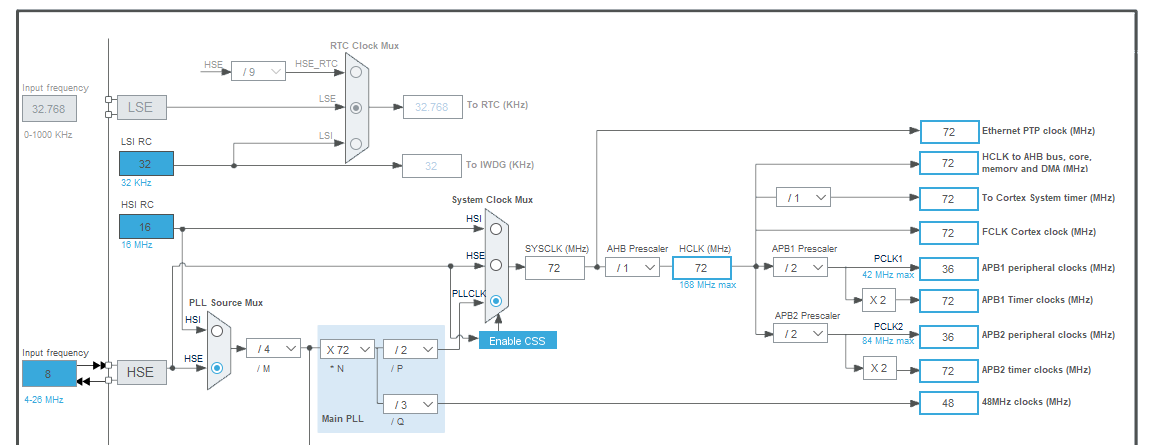
\includegraphics[width = 1\textwidth]{obrazky/CLK_config.png}
        \caption{Clock configuration}
        \label{fig: Clock configuration}
    \end{figure}

    \subsection{Konektivita}
    Ovládací karta je vybavena USB-micro a RJ45 konektorem. Umožňuje tak velmi snadné propojení s PC aplikací
    pomocí standardních USB a ethernetových rozhraní.

    \subsubsection{Ethernet}
    Pro zajištění ethernetového připojení je využito MAC
    vrstvy mikrokontroléru společně s fyzickou vrstvou (PHY)
    realizovanou pomocí čipu DP83848 a RJ45 konektoru s integrovaným transformátorem pro 100 BASE-T. Komunikace mezi
    mikrokontrolérem a DP83848 je realizováno pomocí RMII rozhraní. PHY vyžaduje pro svou správnou funkčnost
    100$\Omega$ diferenciální páry (viz. schéma ovládací karty v příloze).\\
    
    DP83848 vyžaduje pro svou činnost v RMII režimu připojení externího 50\,MHz oscilátoru.
    Výstup oscilátoru je zároveň přiveden na příslušný pin mikrokontroléru a slouží jako 
    hodinová reference.\\ 

    DP83848 je možno konfigurovat pomocí tzv. bootstrap pinů. DP83848 při svém startu zjišťuje
    logické úrovně bootstrap pinů a podle toho konfiguruje své parametry. Následující tabulka
    shrnuje nastavení bootstrap pinů použitých v ovládací kartě.

    \begin{table}[ht!]
        \resizebox{\columnwidth}{!}{%
        \begin{tabular}{|c|c|l|}
        \hline
        \textbf{PIN} & \textbf{Nastavení} & \textbf{Popis}                                   \\ \hline
        AN0 & 1 & AN0 a AN1 piny konfigurují, jakými možnostmi se bude zařízení prezentovat   při AutoNegotioation.   \\ \hline
        AN1 & 1 & Pro kombinaci AN0 = 1 a AN1 = 1 zařízení se prezentuje jako  10BASE-T a 100BASE-TX HALF/FULL duplex \\ \hline
        LED\_CFG     & 1                  & Konfiguruje chování LED na RJ45 konektoru.       \\ \hline
        MII\_MODE    & 1                  & DP83848 očekává RMII pro komunikaci s MAC vrstvou \\ \hline
        MDIX ENABLE  & 1                  & Interní pull up - MDIX (crossover) povolen       \\ \hline
        \end{tabular}%
        }
        \caption{Nastavení bootstrap pinů DP83848}
        \label{RMII settings}
        \end{table}


    Protože ani mikrokontrolér a ani DP83848 nenabízí jedinečnou MAC adresu je použita EEPROM,
    která má již od výrobce naprogramovanou jedinečnou MAC adresu.
    EEPROM používá ke komunikaci I2C protokol a při startu zařízení je MAC adresa
    načtena do MAC vrstvy mikrokontroléru. V mikrokontroléru je implementován telnet
    a http server a je využito LWIP stacku společně s HAL knihovnami a RTOS.\\

    \subsubsection{USB}
    Mikrokontrolér je vybaven fyzickou vrstvou pro USB OTG,
    je tak možné propojit datové signály přímo s USB-micro konektorem.
    Přestože je do USB konektoru vyveden ID pin, který slouží
    k rozlišení mezi host a device, využívá ovládací karta pouze device režim.
    Pro detekci připojení ovládací karty k USB portu je použit napěťový dělič, jehož výstup
    je přiveden do USB\_sense pinu mikrokontroléru. Napěťový dělič obsahuje rezistor o toleranci
    1\,\%. Tuto toleranci není nutno dodržet a tento rezistor byl použit pouze z důvodu nízké ceny
    a faktu, že se již v návrhu vyskytuje.\\

    Připojení pomocí USB slouží převážně k servisním účelům.
    Ovládací kartu lze napájet přímo z USB portu, přičemž napájení je opatřeno
    vstupním filtrem realizovaným feritovou perličkou a kondenzátorem (více v sekci o napájení).
    Obdobně jako u ethernetu je i zde nutno při návrhu PCB použít diferenciální páry
    pro datové signály (90\,$\Omega$). Každý ze signálů,
    který je vyveden na USB-micro konektor je opatřen TVS diodami pro ochranu
    proti ESD. \\

    \begin{figure}[ht!]
        \centering
        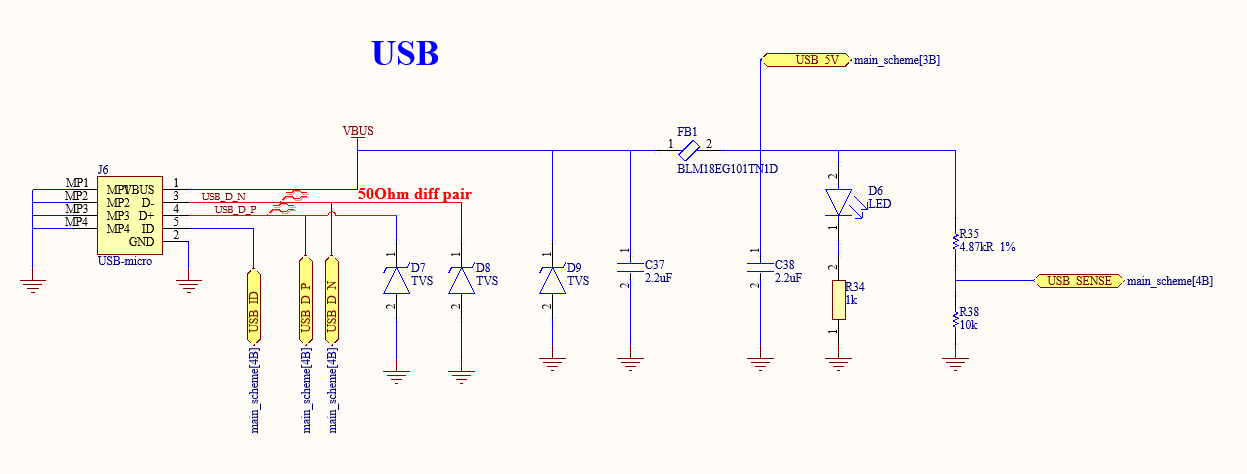
\includegraphics[width = 1\textwidth]{obrazky/USB.png}
        \caption{USB rozhraní}
        \label{fig: USB rozhraní}
    \end{figure}

\clearpage
    \subsection{Napájení}
    Při normálním provozu se počítá s externím napájení v rozmezí 7-15 VDC.
    Toto napětí je přivedeno na WAGO svorky. Napětí (ve schématu BOARD\_PWR)
    přivedeno na vstup nastavitelného regulátoru TLV76701DGNR. Funkce tohoto regulátoru je obdobná
    jako u regulátorů popsaných v sekci o měřící kartě. Výstup regulátoru je možné
    nastavit trimmerem v rozmezí přibližně od 2.8 do 3.45V (ve schématu 3v3\_MCUs).\\

    \begin{figure}[ht!]
        \centering
        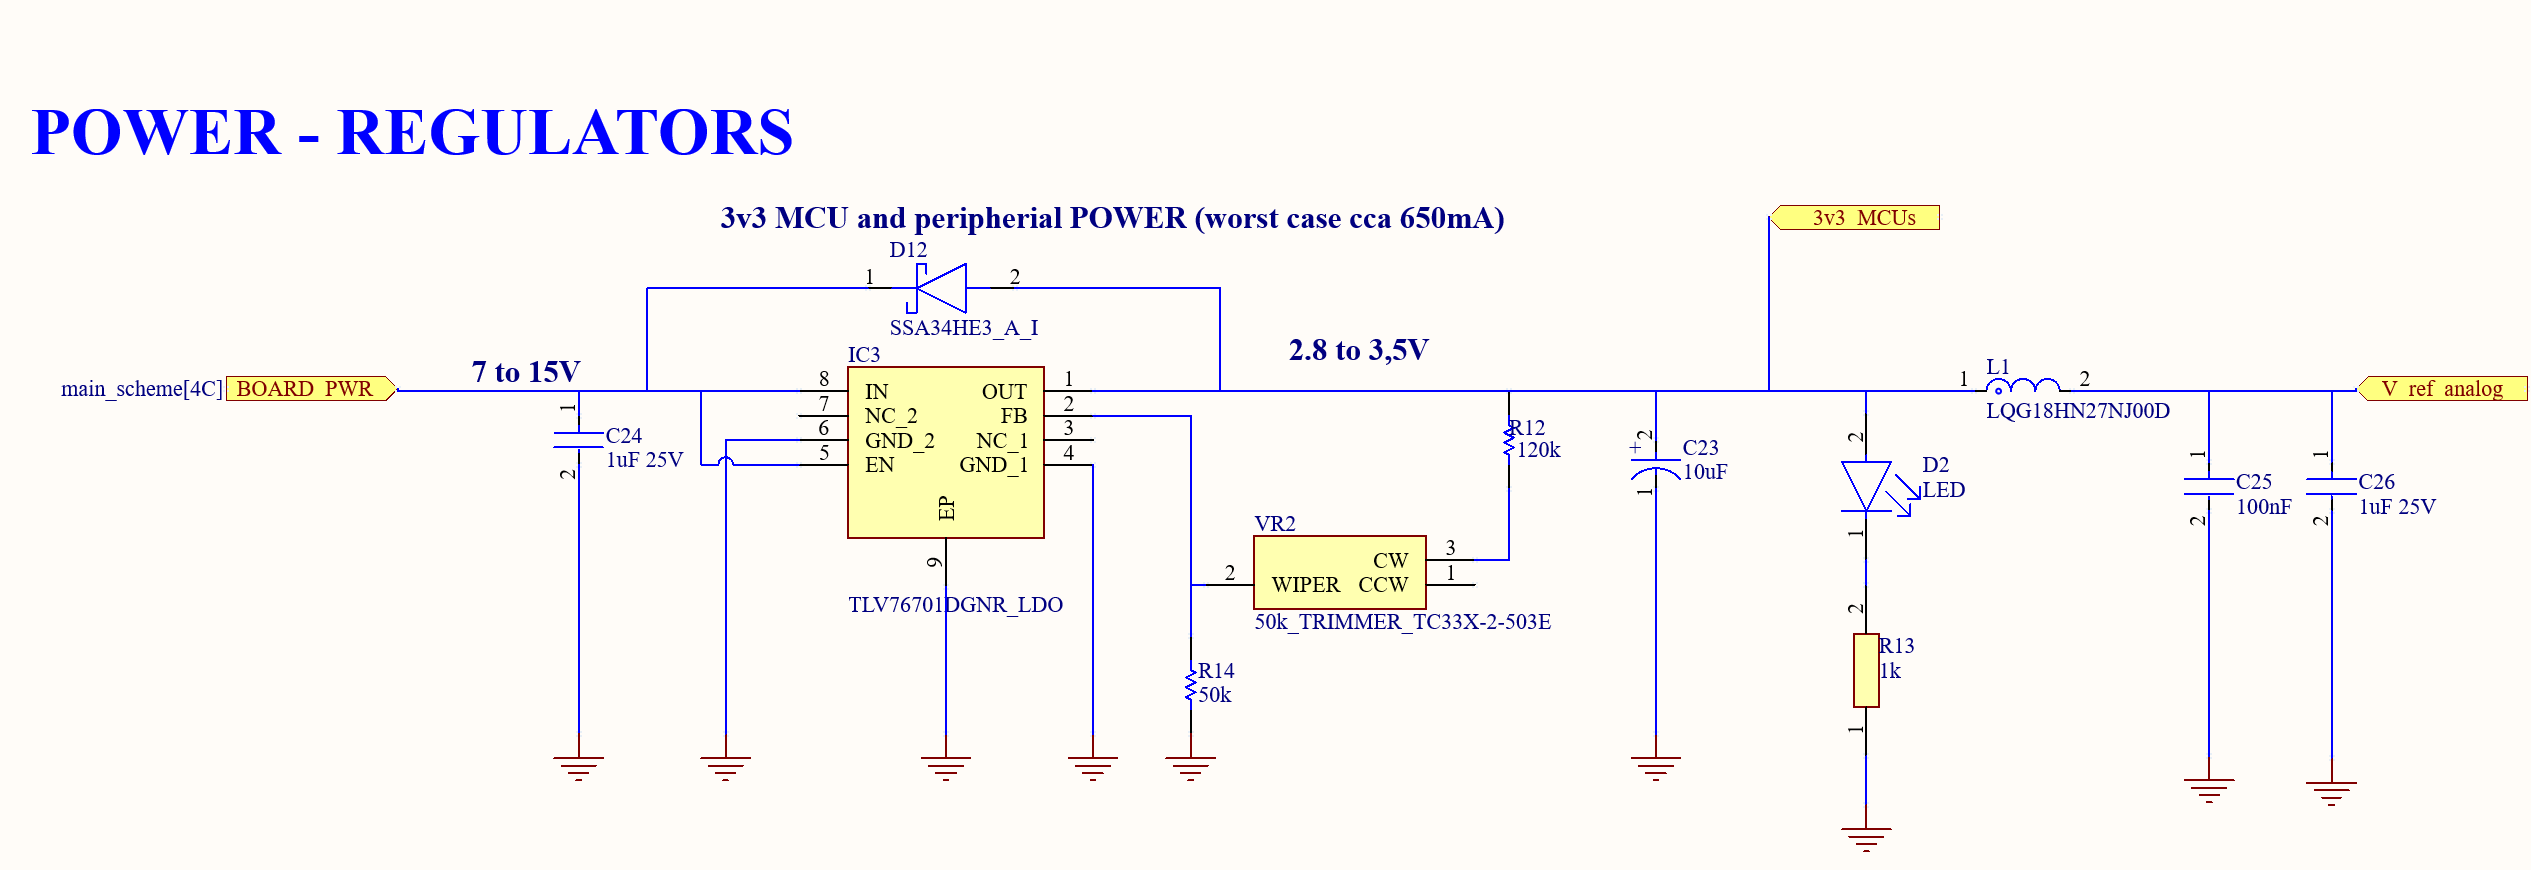
\includegraphics[width = 1\textwidth]{obrazky/PWR_REG_3V3.png}
        \caption{Regulátor napětí - 3V3 MCUs}
        \label{fig:Regulátor napětí - 3V3 MCUs}
    \end{figure}

    Takto regulované napětí je použito pro napájení všech doposud popsaných částí ovládací karty.
    Protože je vhodné aby referenční napětí (V\_ref\_analog),
    které mikrokontrolér používá  pro funkci A/D a D/A převodníků bylo co nejpřesnější, je
    napětí 3V3\_MCUs filtrováno dolní propustí realizovanou pomocí LC filtru.\\

    Očekávaný maximální proud fyzické vrstvy ethernetu je přibližně 150\,mA.
    Proudový odběr ovládací karty nelze jednoznačně určit,
    protože je závislý na firmwaru mikrokontroléru.
    Nicméně se očekává, že by proud v nejhorším případě neměl přesáhnout 500\,mA. 
    Použitý regulátor by měl být schopen dodat do obvodu proud 1A, což by
    mělo být dostačující.\\ 
    
    Napětí je dále přivedeno na 2x25 pinový konektor,
    aby bylo možné napájet měřící a ovládací karty současně připojením napájecí napětí pouze
    na jednu z karet.\\

    Celý systém měřících a ovládacích karet může být napájen pomocí USB. V tomto případě je však přesnost
    měření limitována kvalitou USB napájení. Následující obrázek znázorňuje distribuci napájení
    ovládacích a měřících karet. Schéma však neodpovídá reálnému zapojení, protože jednotlivé
    komponenty jsou propojeny přes 2x25 pin konektory. Pro přehlednost jsou však konektory vynechány.
    \clearpage


    \begin{figure}[ht!]
        \centering
        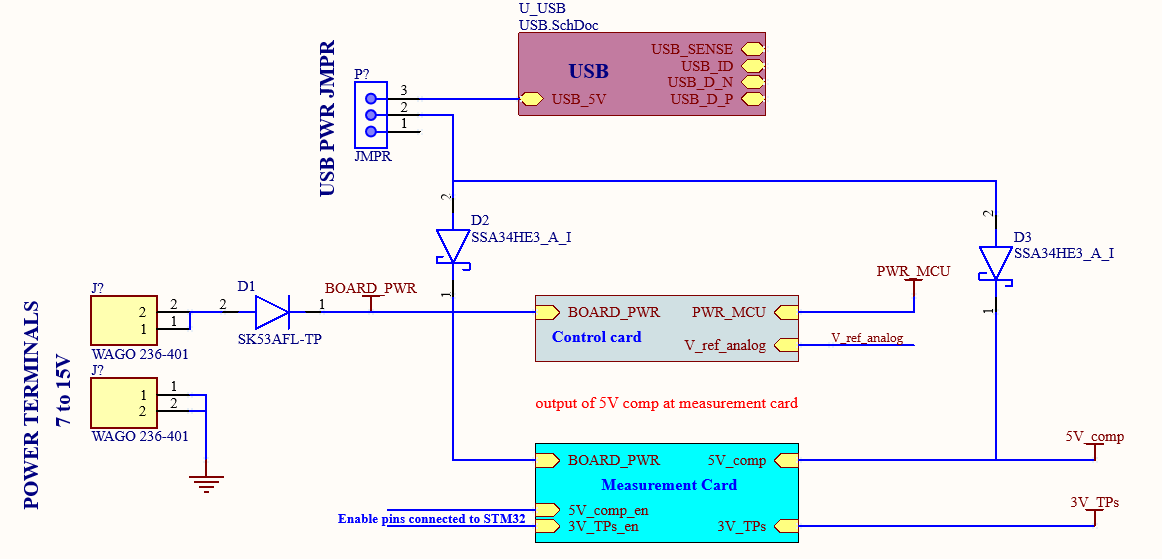
\includegraphics[width = 1\textwidth]{obrazky/USB_power_distr.png}
        \caption{Distribuce napájení}
        \label{fig:Distribuce napájení}
    \end{figure}

    V případě napájení pomocí USB je napětí BOARD\_PWR generováno z USB portu.
    Aby se zamezilo poškození všech připojených zařízení, které by mohlo potenciálně vzniknout připojením
    vyššího napětí na WAGO svorkách a USB současně, je do schématu připojena dioda D2. Dioda D1
    slouží jako ochrana k přepólování na vstupu WAGO svorek. Zároveň dioda D1 plní obdobnou funkci jako dioda D2
    nyní však pro ochranu zdroje napájení připojeného do WAGO svorek proti napětí na USB.
    V případě současného připojení externího napětí na WAGO svorky a USB portu, bude deska napájena
    vyšším z napětích.\\

    Napětí BOARD\_PWR je v případě napájení přes USB rovno přibližně:
    
    \begin{equation}
        V_{BOARD\_PWR} = V_{USB} - V_{D2} = 5V - 0.4V = 4.6V,
    \end{equation}
    Kde $V_{D2}$ je úbytek na diodě D2. Tento úbytek je pro diodu SSA34HE3\_A\_I roven přibližně 0.2V při proudu 1A
    a přibližně 0.4V při proudu 2A\\

    Úbytek napětí na regulátorech TLV76701DGNR je přibližně 0.8V.
    Součtem úbytků na diodě D2 a regulátoru lze 
    dosáhnou regulovaného výstupního napětí až 3.8V, což je dostatečné pro napájení všech regulátorů
    kromě regulátoru, který zajišťuje napětí 5V\_comp. Napětí 5V\_comp je tedy generováno přímo z USB portu přes 
    diodu D3. Dioda D3 má obdobný význam jako dioda D2, nyní však chrání USB port před vyšším napětím na výstupu
    regulátoru 5V\_comp v případě napájení z WAGO svorek. Z tohoto je patrné, že napětí 5V\_comp není nijak regulováno
    a je přímo závislé na napětí a rušení USB portu.
    V případě detekce napětí na USB\_sense pinu je komparátor 5V\_comp vypnut pomocí enable pinu.\\

    Pro možnost použití USB rozhraní pouze pro komunikaci (ne pro napájení),
    lze USB napájení rozpojit pomocí jumperu.\\

    





    %\subsection{Návrh PCB}
    %Tady bude sekce o návrhu PCB. Zatím není navrženo.
    %Ve výrobě jsou měřící karty, které by snad i s osazením měly být hotové do obhajoby semestrální práce.
    %Poté bude měřící karta otestována jejich funkčnost pomocí NUCLEO prototypových kitů.
    %Po verifikaci funkčnosti bude vyrobena ovládací karta.
    %Bude se pravděpodobně jednat o šestivrstvé PCB s řízenými impedancemi pro diferenciální páry.
    %    \subsubsection{USB routing}
    %Nějaký stručný popis vlivu impedance cesty na rychlost USB...
    %\subsubsection{Ethernet routing}
    %Nějaký stručný popis vlivu impedance cesty na rychlost Ethernetu. Signal integrity atd..
    %\subsubsection{STM32F4 routing}
    %Vliv decoupling kondenzátorů.
    %\subsubsection{Fyzické rozměry}
    %Na rozdíl od měřících karet, kde byl kladen důraz na maximální výšku karty z důvodu roztečí bRC pinů, nejsou
    %kladeny na ovládací karty žádné omezení, protože ovládací karty budou propojeny s měřícími kartami
    %pomocí páskových vodičů. Rozměry by však měly být co nejkompaktnější. Propojit měřící karty s bRC piny pomocí
    %páskových vodičů nebylo žádoucí z důvodu vnášení chyby měření do systému.
    %\clearpage


\chapter{Algoritmizace a měřící procedury}
Jak již bylo zmíněno v kapitole o systémové koncepci a na obr.\ref{fig:Systémová koncepce}.
Jednotlivé ovládací karty jsou propojeny pomocí ethernetového rozhraní do switche.
Pro správnou funkčnost testeru je zde použit spravovatelný switch, který mimo jiné umožňuje
získat informace o své MAC tabulce. MAC tabulku společně s protokolem ARP lze využít pro
přiřazení čísla portu ethernetového switche k IP adrese připojených ovládacích karet. Tímto způsobem
lze přiřadit jednotlivé ovládací karty k jednotlivým řadám bRC pinů bez nutnosti dodatečné konfigurace
či různému kódování řad.\\

Z pohledu celého systému je hlavním řídícím prvkem PC aplikace. V následující části je popsán Komunikační
protokol, který je použit pro komunikaci mezi PC aplikací a ovládacími kartami.

\section{Komunikační protokol ovládacích karet}
Komunikační protokol je založen na ASCII příkazech a je tak relativně čitelný pro člověka.
Jednotlivé příkazy protokolu jsou přenášeny pomocí TCP/IP rámců (port 23) v případě ethernetového rozhraní nebo
pomocí Virtuálního COM portu v případě USB rozhraní. Pro obě možnosti připojení se protokol neliší.\\

Jednotlivé příkazy jsou vyhodnocovány po obdržení znaku CR (ASCII 0x0D), LF (ACII 0x0A) popřípadě libovolnou kombinací těchto znaků. Odpovědi
z ovládacích karet jsou zakončeny znakem LF. Ovládací karta je určena obecně k ovládání více modulů než pouze měřících karet. Nicméně pro účely
diplomové práce jsou diskutovány pouze příkazy vztahující se k měřícím kartám. Každý příkaz vztahující se k měřícím kartám obsahuje prefix 80\_IO\_CARD.
Jednotlivé parametry příkazu jsou odděleny mezerou.\\

Pro každý příkaz odesílá ovládací karta odpovědi začínajícími prefixem "ERROR;" nebo "OK;" (bez uvozovek) podle toho, zda-li byl příkaz vyhodnocen úspěšně či nikoliv.
Poté následuje textová odpověď na příkaz zakončená znakem LF.
Příkazy jsou obecně rozděleny do 3 skupin (SET READ a MEASUERE). Skupina SET slouží k nastavení parametrů měření, skupina READ slouží k čtení nastavených parametrů
a skupina MEASURE slouží k samotnému měření.\\

V následujicích podkapitolách jsou popsány jednotlivé příkazy pomocí následující konvence:
\begin{itemize}
    \item Znak | značí, že je možné použít pouze jeden z uvedených parametrů.
    \item Text v uvozovkách značí nastavitelnou hodnotu do příkazu se zadává bez uvozovek a v případě desetinných čísel je použita destinná tečka.
    \item Text mezi * je vysvětlen podrobněji v dané sekci
    
\end{itemize}

\subsection{Příkazy SET}
\subsubsection{SET DAC}
Příkaz SET DAC slouží k nastavení napětí na výstupu DAC. Protože se jedná o 12 bitový převodník, je možné nastavit pouze hodnoty napětí, které jsou násobky
napětí referenčního napětí. Pokud je zadáno napětí, které není násobkem referenčního napětí, je nastaveno nejbližší nižší napětí.
Referenční napětí ovládací karty je nastaveno při kalibraci příkazem SET CONFIGURATION VOLTAGE\_REFERENCE. Případně je hodnotu referenčního napětí možno získat
příkazem READ CONFIGURATION VOLTAGE\_READINGS.
\begin{itemize}[leftmargin=*]
    \item \textbf{Obecný tvar:} 80\_IO\_CARD SET DAC "Napětí ve V"
    \item \textbf{Příklad:}\\
    -> 80\_IO\_CARD SET DAC 2.75\\
    <- OK;DAC: 3398, discretized Value in Volts:2.74959
    \item \textbf{Interpretace odpovědi:} Tato odpověď byla obdržena při referenčním napětí 3.314400V. Hodnota 3398 je bitová hodnota, která je zapsána do registru DAC a
    hodnota 2.74959 je odpovídající hodnota napětí.
\end{itemize}

\subsubsection{SET SHIFT\_REGISTER}
Příkaz SET SHIFT\_REGISTER slouží k nastavení výstupní hodnoty posuvného registru či celé skupiny posuvných registrů.
Prvním parametrem příkazu je volba skupiny posuvných registrů.
Relevantní skupiny posuvných registrů pro diplomovou práci jsou IO1TO40\_OUTPUTS, IO41TO80\_OUTPUTS, IO1TO40\_IMPEDANCES a IO41TO80\_IMPEDANCES.
Správnou kombinací výstupů těchto posuvných registrů lze nastavit jakýkoliv bRC pin do vysoké či nízké impedance a případně i výstupní hodnotu napětí.\\

Druhým parametrem je volba způsobu zadání výstupní hodnoty registrů. K dispozici jsou následující možnosti: VALUE a DO\_N\_SHIFTS.
V případě možnosti VALUE následuje decimální hodnota jejíž bitové vyjádření reprezentuje stavy jednotlivých výstupů posuvných registrů.
Každý ze skupin registrů má svoji endianitu, kterou lze zjistit z příkazu READ CONFIGURATION SHIFT\_REGISTERS (podrobněji popsáno dále). 
Druhý způsob je DO\_N\_SHIFTS, který posune celý obsah posuvného registru o zadaný počet bitů v pravo či vlevo v závislosti na endianitě registru.

\begin{itemize}[leftmargin=*]
    \item \textbf{Obecný tvar:} 80\_IO\_CARD SET SHIFT\_REGISTER *registr* *způsob* "Hodnota"
    \item \textbf{*registr*:} IO1TO40\_OUTPUTS, IO41TO80\_OUTPUTS,\\
    IO1TO40\_IMPEDANCES, IO41TO80\_IMPEDANCES
    \item \textbf{*způsob*:} VALUE, DO\_N\_SHIFTS
    \item \textbf{Příklad:}\\
    -> 80\_IO\_CARD SET SHIFT\_REGISTER IO1TO40\_IMPEDANCES VALUE 4\\
    <- OK;Setting Register:IO1TO40\_IMPEDANCES to:4\\
    -> 80\_IO\_CARD SET SHIFT\_REGISTER IO1TO40\_IMPEDANCES DO\_N\_SHIFTS 4\\
    <- OK;Setting Register:IO1TO4\_IMPEDANCES to:16
    \item \textbf{Interpretace odpovědi:} Obecně lze vždy v odpovědi nalézt nový stav registru po provedení požadované operace.
\end{itemize}

\subsubsection{SET CONFIGURATION}
Příkazy v této skupině obecně slouží k nastavení stavových hodnot, kalibračních hodnot případně nastavení způsobu
měření určitých hodnot. Hodnoty, které potřebují být nastaveny pomocí prefixu SET CONFIGURATION jsou popsány v sekcích pro které jsou tyto hodnoty používány.
Ukázky vybraných hodnot, které lze nastavit pomocí příkazu SET CONFIGURATION jsou uvedeny například v sekci READ CONFIGURATION.

\begin{itemize}[leftmargin=*]
    \item \textbf{Obecný tvar:} 80\_IO\_CARD SET CONFIGURATION *Název konfigurace* "Hodnota"
    \item \textbf{*Název konfigurace*:} Popsáno v sekcích pro které jsou hodnoty používány.
    \item \textbf{Příklad:}\\
    -> 80\_IO\_CARD SET CONFIGURATION VOLTAGE\_REFERENCE 3.3144\\
    <- OK;VOLTAGE\_REFERENCE set to:3.314400
    \item \textbf{Interpretace odpovědi:} Obecně lze vždy v odpovědi nalézt potvrzení o nastavení hodnoty.
\end{itemize}

\subsection{Příkazy READ}
\subsubsection{READ MUX}
Příkaz READ MUX umožňuje číst hodnoty z multiplexerů umístěných na ovládací kartě. Příkaz se zkládá ze 2 parametrů. Prvním parametrem je volba
skupiny multiplexerů. Pro ovládací kartu jsou k dispozici 2 skupiny (MUXES\_1TO40 a MUXES\_41TO80). Druhým parametrem je volba podoby obdržené hodnoty.
První možností je přečíst hodnotu celé skupiny multiplexeru za použití parametru ALL. Výsledkem tohoto příkazu je 40bitové číslo v decimální podobě,
kde každý bit reprezentuje stav jednoho bRC pinu připojeného ke zvolenému multiplexeru. 40biová hodnota je vztažena k endianitě multiplexeru, kterou lze zjistit
příkazem 80\_IO\_CARD READ CONFIGURATION MULTIPLEXERS.
Druhou možností je zadat přímo číslo pinu, jehož stav chceme zjistit. Výsledkem tohoto příkazu je 1bitová hodnota v decimální podobě.
\begin{itemize}[leftmargin=*]
    \item \textbf{Obecný tvar:} 80\_IO\_CARD READ MUX *multiplexer* "číslopinu"|ALL
    \item \textbf{*multiplexer*:} MUXES\_1TO40 a MUXES\_41TO80
    \item \textbf{Příklad:}\\
    -> 80\_IO\_CARD READ MUX MUXES\_1TO40 ALL\\
    <- OK;Reading MUX MUXES\_1TO40, ALL:0\\
    -> 80\_IO\_CARD READ MUX MUXES\_1TO40 1\\
    <- OK;Reading MUX: MUXES\_1TO40, address:1, value:0
    \item \textbf{Interpretace odpovědi:} V případě parametru ALL je v odpovědi obsažena 40bitová hodnota v decimální podobě. V případě zadání čísla pinu je v odpovědi obsažena 1bitová hodnota v decimální podobě.
\end{itemize}

\subsubsection{READ SHIFT\_REGISTER}
Tento příkaz slouží k získání aktuální hodnoty shiftregistru. Jediným parametrem tohoto příkazu je jméno skupiny shiftregistru.

\begin{itemize}[leftmargin=*]
    \item \textbf{Obecný tvar:} 80\_IO\_CARD READ MUX *register*
    \item \textbf{*register*:} IO1TO40\_OUTPUTS, IO41TO80\_OUTPUTS,\\
    IO1TO40\_IMPEDANCES, IO41TO80\_IMPEDANCES
    \item \textbf{Příklad:}\\
    -> 80\_IO\_CARD READ SHIFT\_REGISTER IO1TO40\_OUTPUTS\\
    <- OK;Reading Register IO1TO40\_OUTPUTS, value:1099511627775\\
    \item \textbf{Interpretace odpovědi:} V odpovědi je obsažena 40bitová hodnota v decimální podobě,
    kde jednotlivé bity této hodnoty značí aktuální výstupní hodnotu shiftregistru v závislosti na jeho endianitě.
    V případě výpadku napájení se může stát, že hodnota shiftregistru nebude odpovídat skutečnému stavu výstupních pinů.
\end{itemize}


\subsubsection{READ CONFIGURATION}
Příkaz READ CONFIGURATION slouží k získání konfigurace ovládací karty. Ovládací karta obsahuje poměrně obsáhlé množství konfigurací.
V této sekci jsou popsány pouze ty konfigurace, které jsou využívány v diplomové práci. Některé vyčtené tímto příkazem nastavovat
pomocí příkazu SET CONFIGURATION.
\begin{itemize}[leftmargin=*]
    \item \textbf{Obecný tvar:} 80\_IO\_CARD READ CONFIGURATION *konfigurace*
    \item \textbf{Příklad SHIFT\_REGISTERS:}\\
    -> 80\_IO\_CARD READ CONFIGURATION SHIFT\_REGISTERS\\
    <- OK;IO1TO40\_OUTPUTS:(length:40,endianity:1,value:1099511627775);\\
    IO41TO80\_OUTPUTS:(length:40,endianity:0,value:0);\\
    IO1TO40\_IMPEDANCES:(length:40,endianity:1,value:1);\\
    IO41TO80\_IMPEDANCES:(length:40,endianity:0,value:0);
    \item \textbf{Interpretace odpovědi:} V odpovědi jsou obsaženy veškeré informace o konfiguraci posuvných registrů.
    \item \textbf{Příklad MULTIPLEXERS:}\\
    -> 80\_IO\_CARD READ CONFIGURATION MULTIPLEXERS\\
    <- OK;MUXES\_1TO40:(bits:8,paralel:5,endianity:0,value:0);\\
    MUXES\_41TO80:(bits:8,paralel:5,endianity:0,value:0);
    \item \textbf{Interpretace odpovědi:} V odpovědi jsou obsaženy veškeré informace o konfiguraci multiplexerů.
    \item \textbf{Příklad VOLTAGE\_READINGS:}\\
    -> 80\_IO\_CARD READ CONFIGURATION VOLTAGE\_READINGS\\
    <- OK;DAC\_RAMP\_DIRECTION:0;\\
    DAC\_RAMP\_MIN\_VALUE\_VALUE:0;\\
    DAC\_RAMP\_MAX\_VALUE\_VALUE:4095;\\
    DAC\_RAMP\_STEP:1;\\
    DAC\_RAMP\_DELAY\_2500\_NS:2;\\
    VOLTAGE\_READ\_AVERAGES:2;\\
    VOLTAGE\_REFERENCE:3.314400;
    \item \textbf{Interpretace odpovědi:} V odpovědi jsou obsaženy veškeré nastavitelné parametry, které se využívají při měření napětí na jednotlivých pinech příkazy MEASURE.
\end{itemize}





\subsection{Příkazy MEASURE}
\subsubsection{MEASURE VOLTAGE}
Příkaz MEASURE VOLTAGE slouží k měření napětí na určitém bRC pinu či pinech. V případě použití parametru ALL je změřeno napětí na všech 80 pinech měřící karty.
V případě, že je místo parametru ALL zadáno číslo tak příkaz vrátí hodnotu napětí na daném pinu.\\

\begin{itemize}[leftmargin=*]
    \item \textbf{Obecný tvar:} 80\_IO\_CARD MEASURE VOLTAGE ALL|"číslo pinu"
    \item \textbf{Příklad ALL:}\\
    -> 80\_IO\_CARD MEASURE VOLTAGE ALL\\
    <- OK;2.965643;2.860450;2.431585;-1.000000;0.922465;........;-1.00000;-1.000000;
    \item \textbf{Interpretace odpovědi:} V odpovědi jsou obsaženy hodnoty napětí na všech 80 pinech odděleny znakem ;. "...." V příkladu značí, že výpis byl zkrácen.
    Hodnota -1 značí, že napětí je mimo rozsah měřící karty.

    \item \textbf{Příklad číslo pinu:}\\
    -> 80\_IO\_CARD MEASURE VOLTAGE 3
    <- OK;Voltage:2.128143\\
    \item \textbf{Interpretace odpovědi:} V odpovědi je obsaženo napětí na pinu 3 (číslováno od 0). V případě, že napětí je mimo rozsah měřící karty, tak příkaz vrátí hodnotu -1.
\end{itemize}

Proces měření napětí lze konfigurovat pomocí příkazů ze skupiny SET CONFIGURATION. Následující část popisuje vliv vybraných parametrů.
Měření napětí probíhá pomocí porovnávání nastavené hodnoty D/A převodníku s měřenou hodnotou napětí na bRC pinu. V reálném zapojení je tohoto dosaženo pomocí komparátoru.
Výstup komparátoru je z důvodu velkého množství pinů multiplexován na digitální vstup mikrokontroléru (Obr.\ref{fig: bRC pin voltage measurement}). 

\begin{figure}[ht!]
    \centering
    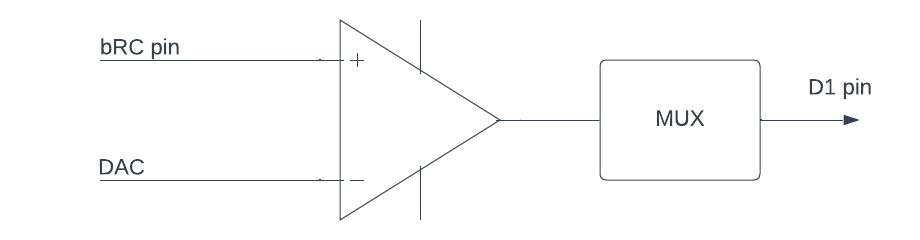
\includegraphics[width = 0.9\textwidth]{obrazky/Voltage_measurement_example.png}
    \caption{Zjednodušené schéma zapojení pro měření napětí na bRC pinu}
    \label{fig: bRC pin voltage measurement}
\end{figure}

Měření popsána v této sekci byla provedena na reálné měřící kartě, kde výstup multiplexeru pro měřený bRC pin je přivedenen na pin D1 olvádací karty. Měření byla provedena pomocí
osciloskopu KEYSIGHT DSOX1204A a digitánlního 6 a 1/2 místného multimetru. Kde jednotlivé průběhy napětí jsou následně zpracovány pomocí programu MATLAB.\\

Na obrázku \ref{fig: bRC pin voltage measurement DACRAMP1} je zobrazen průběh napětí jednotlivých uzlů z obr. \ref{fig: bRC pin voltage measurement}. Modře je znázorněna měřená hodnota napětí na bRC pinu,
která má podle multimetru hodnotu 2.1475V, příčemž příkaz vrátil hodnotu napětí 2.1275V. Tato hodnota je závislá na nastavení napěťové reference příkazem 80\_PIN\_CARD SET CONFIGURATION VOTAGE\_REFERENCE.\\

Červeně je zobrazena hodnota napětí na výstupu D/A převodníku a zeleně je znázorněn výstup multiplexeru. 
Každá z následujících diskutovaných konfigurací v této sekci začíná prefixem 80\_PIN\_CARD SET CONFIGURATION, přičemž je tento prefix vynecháván.

\begin{figure}[ht!]
    \centering
    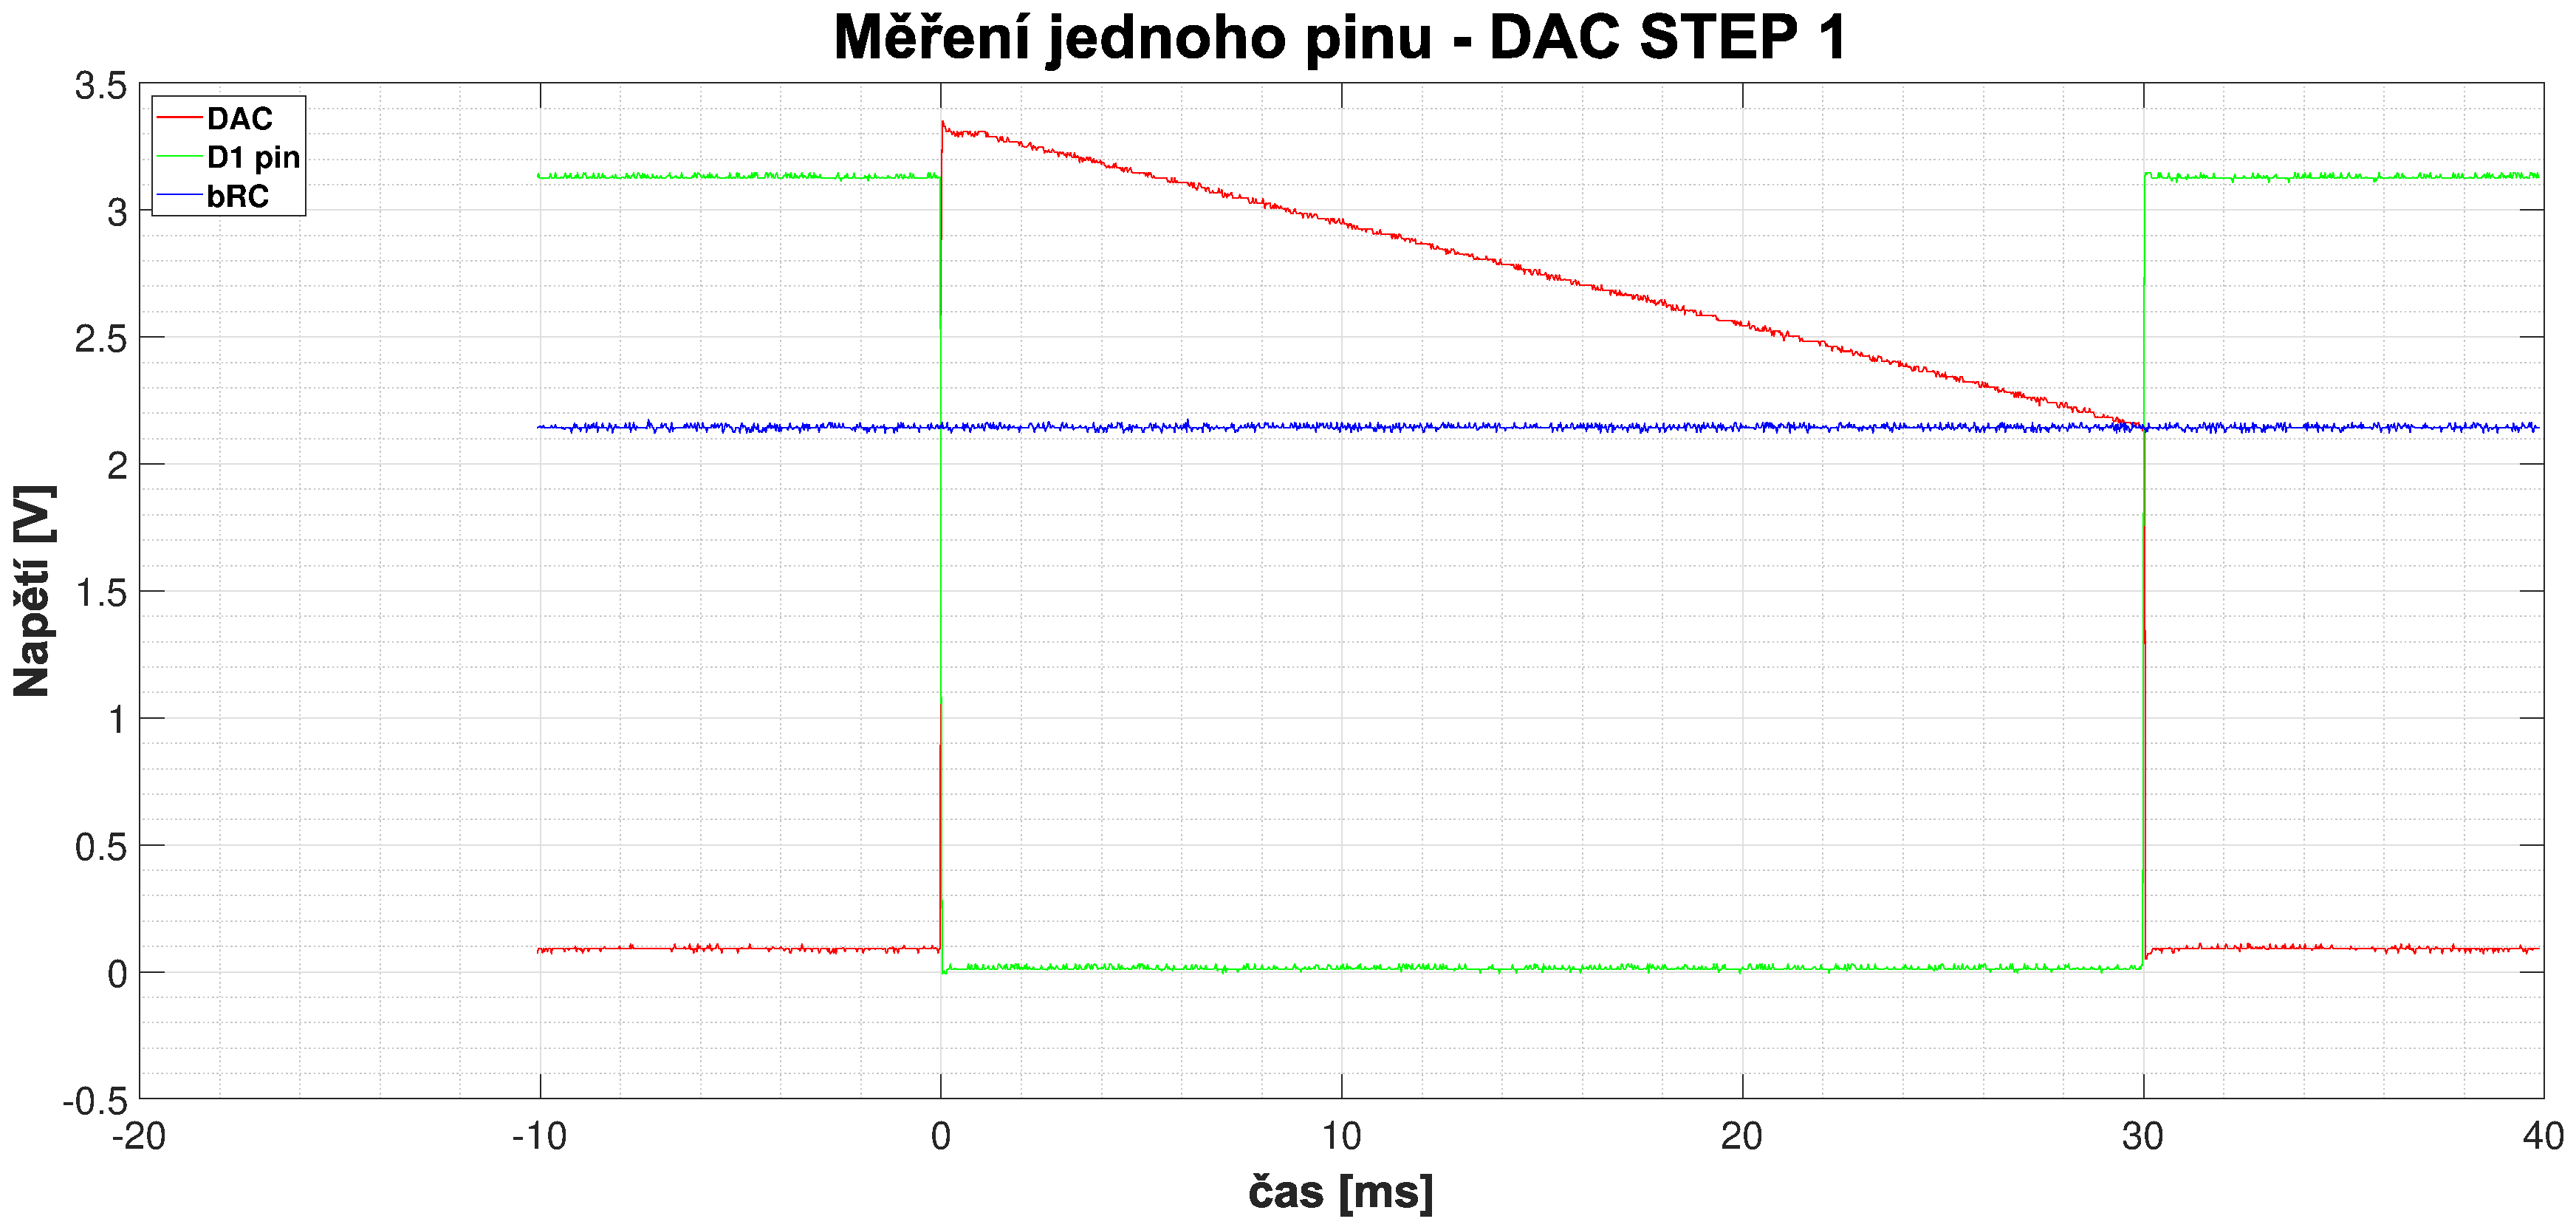
\includegraphics[width = 0.9\textwidth]{obrazky/matlab_generated/pin_step1.eps}
    \caption{Časové průběhy napětí - měření napětí na bRC pinu (DAC\_RAMP = 1)}
    \label{fig: bRC pin voltage measurement DACRAMP1}
\end{figure}

Měření napětí probíhá tak, že se na D/A převodníku nastavují sestupně (případně vzestupně v závislosti na konfiguraci DAC\_RAMP\_DIRECTION) hodnoty napětí. Při každém kroku se kontroluje,
zda nedošlo k překlopení napěťové úrovně na výstupu komparátoru (respektive multiplexeru - D1 pin).
Detekce překlopení probíhá tak, že se vyčítá N-krát (lze nastavit konfigurací VOLTAGE\_READ\_AVERAGES) logická hodnota na pinu D1.
Pokud je alespoň polovina z takto vyčtených hodnot opačné logické úrovně než logická úroveň pinu D1 na počátku měření,
tak se přepočte aktuálně nastavená hodnota registru D/A převodníku na napětí a toto napětí se odešle do PC aplikace.
Detekce překlopení komparátoru je patrná na obrázku \ref{fig: bRC pin voltage measurement DACRAMP1}
přibližně v čase 30\,ms.

\begin{figure}[ht!]
    \centering
    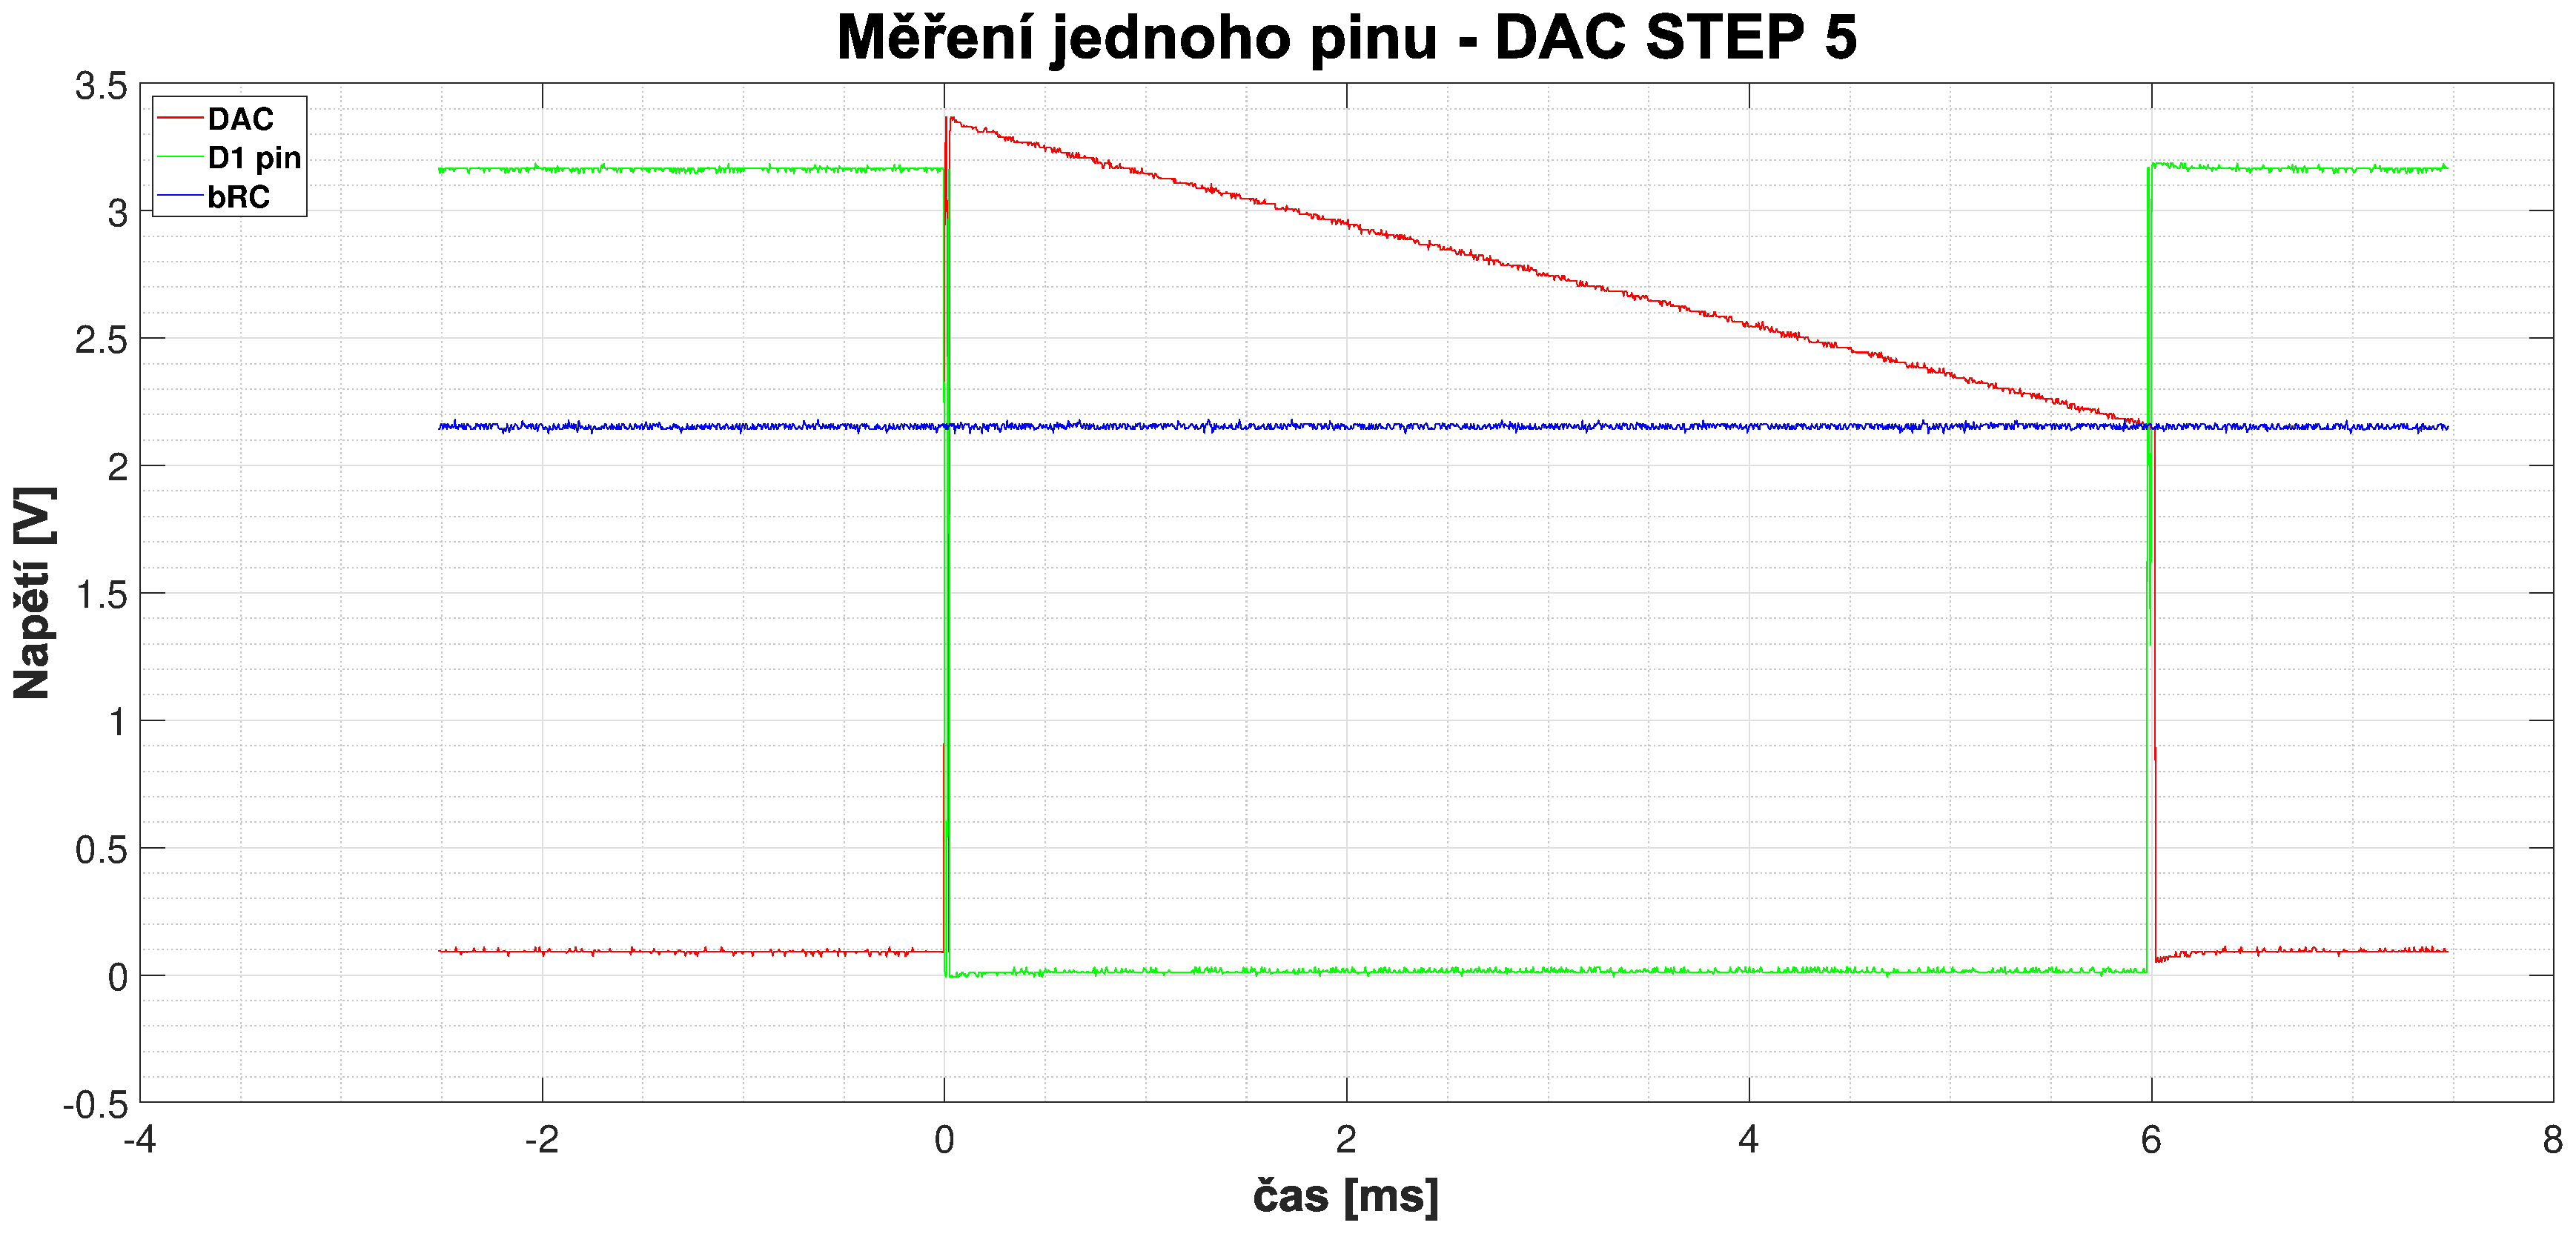
\includegraphics[width = 0.9\textwidth]{obrazky/matlab_generated/pin_step5.eps}
    \caption{Časové průběhy napětí - měření napětí na bRC pinu (DAC\_RAMP = 5)}
    \label{fig: bRC pin voltage measurement DACRAMP5}
\end{figure}

Další nastavitelnou konfigurací je DAC\_RAMP\_STEP, která udává bitový krok rampy D/A převodníku. Takto lze měření urychlit za cenu snížení přesnosti.
Na obrázku \ref{fig: bRC pin voltage measurement DACRAMP5} je zobrazen průběh napětí při nastavení DAC\_RAMP\_STEP = 5. Touto změnou
bylo dosaženo změření stejného napětí jako v předchozím bodě přibližně za 6\,ms.\\

Z obrázků \ref{fig: bRC pin voltage measurement DACRAMP1} a \ref{fig: bRC pin voltage measurement DACRAMP5} lze dedukovat, že celkový čas je závislý 
na měřeném napětí. V případě, že je zvolena sestupná rampa a měřené napětí je nulové budou průběhy vypadat následovně:

\begin{figure}[ht!]
    \centering
    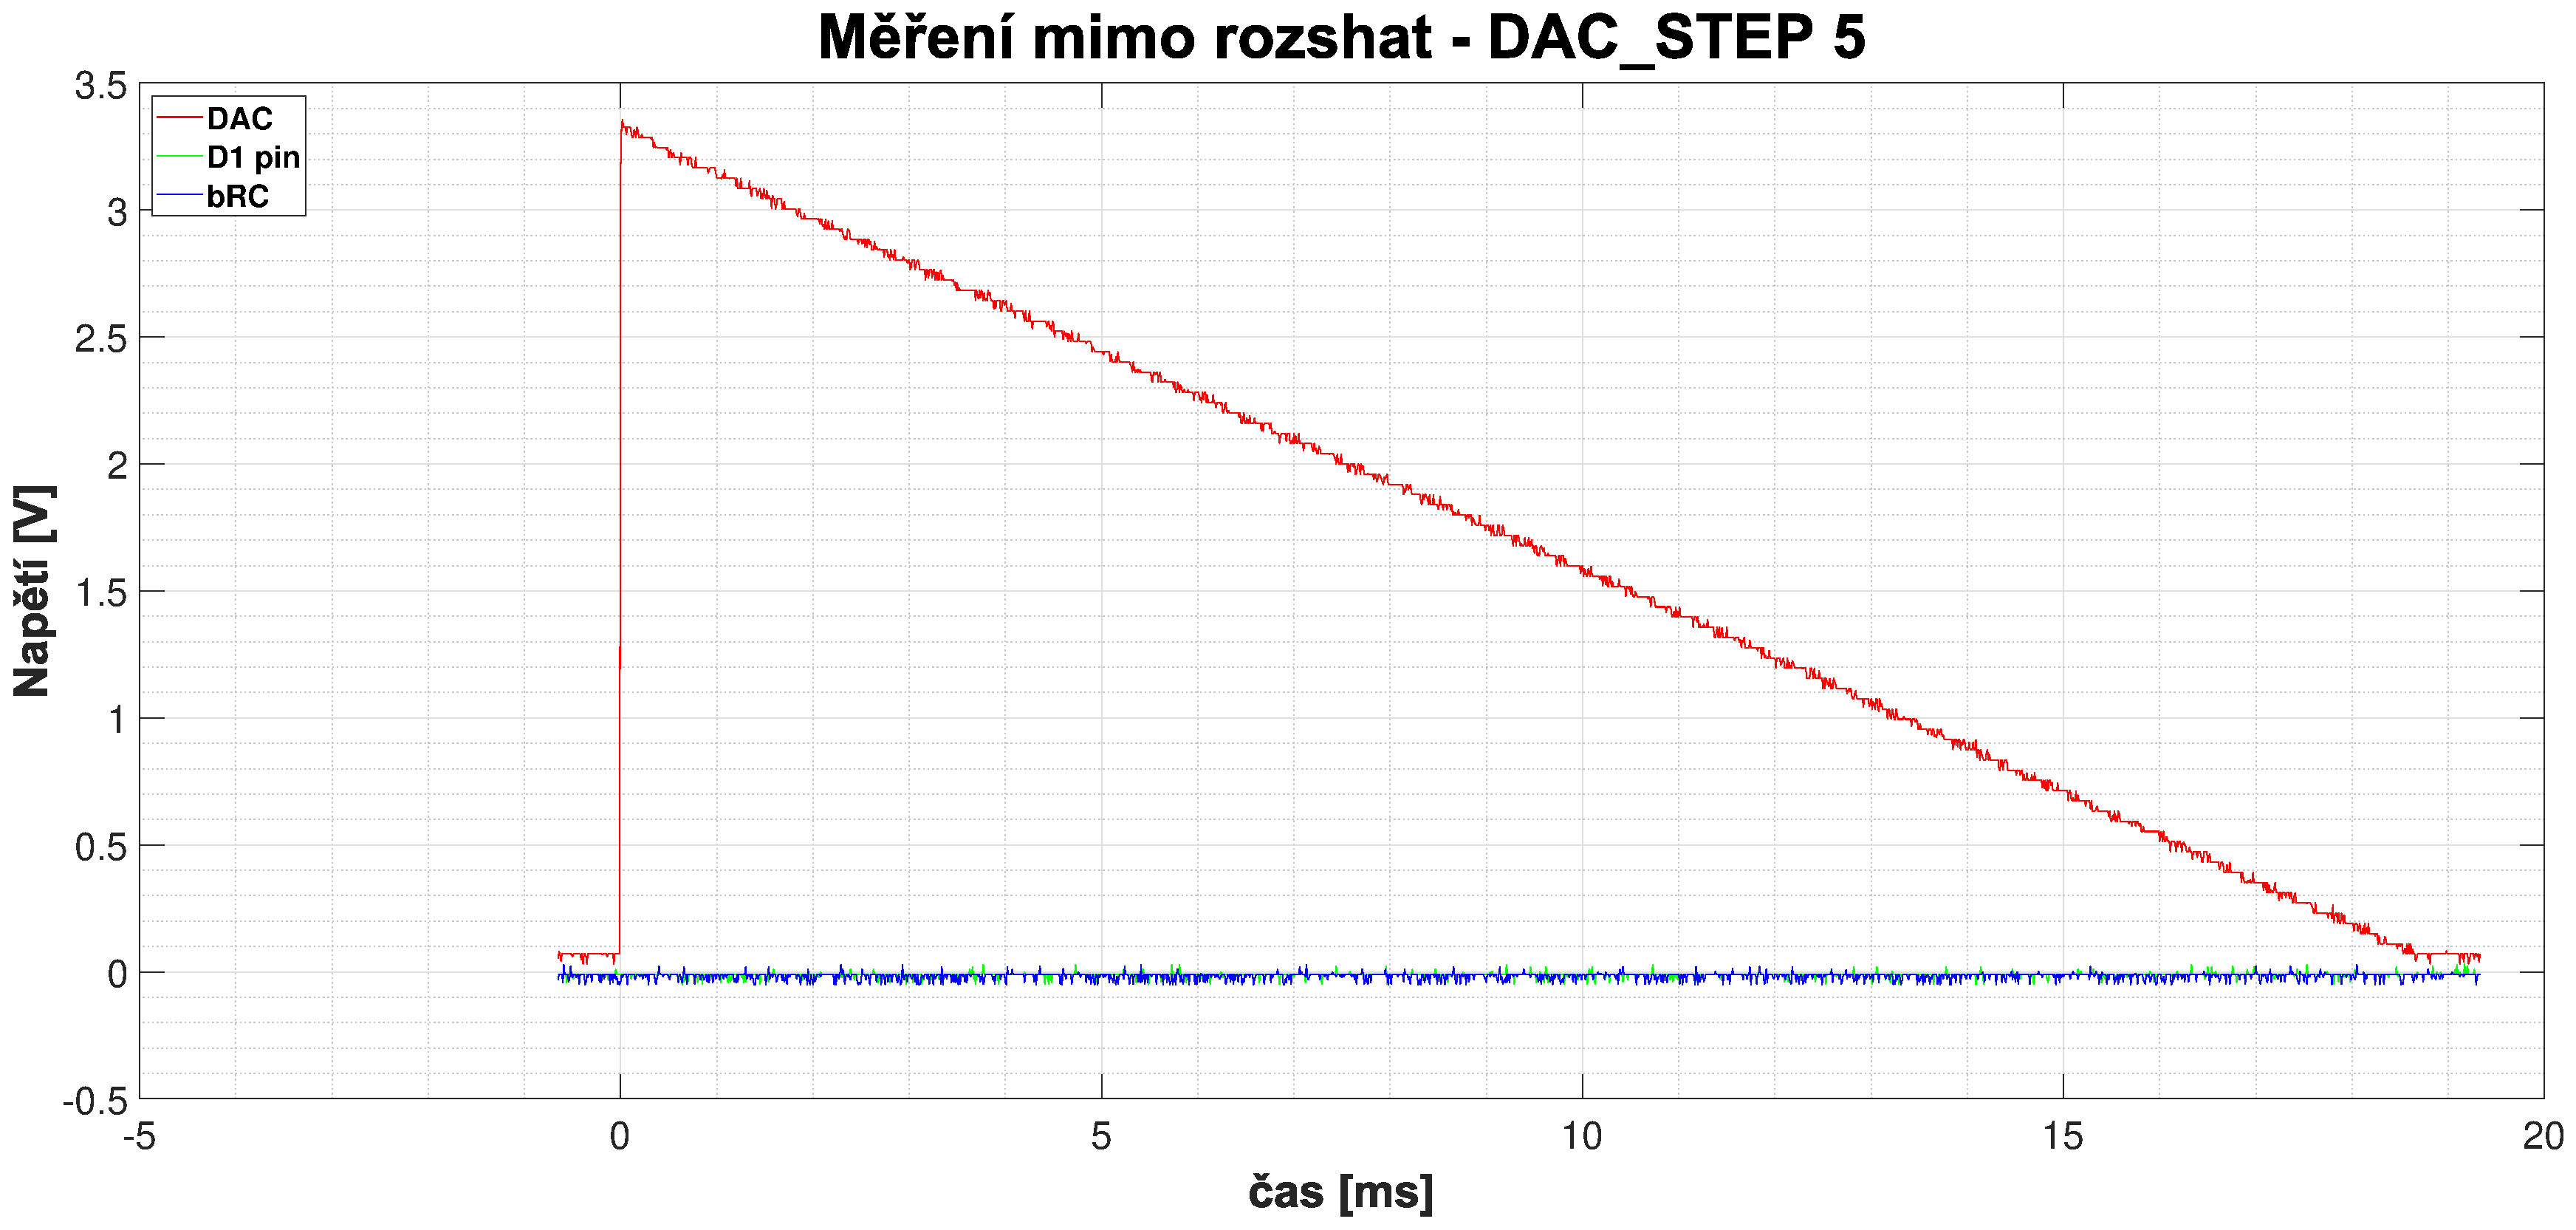
\includegraphics[width = 0.9\textwidth]{obrazky/matlab_generated/pin_out_of_range.eps}
    \caption{Časové průběhy napětí - měření nízkého napětí na bRC pinu (DAC\_RAMP = 5)}
    \label{fig: bRC pin voltage measurement low Voltage}
\end{figure}

Na obrázku \ref{fig: bRC pin voltage measurement low Voltage} lze pozorovat, že pokud napětí je příliš nízké, tak se výstup komparátoru nikdy nepřeklopí a 
příkaz vrátí v odpovědi hodnotu -1.
To je způsobeno tím, že D/A převodník není schopen generovat nulové napětí. Při nastavení registru D/A převodníku na 0 je na výstupu převodníku napětí přibližně 70\,mV.
Lze tak měřit pouze napětí, které je vyšší než tato dolní mez. Horní mez měření není omezena, protože napájecí napětí bRC pinů je nižší než napětí,
které je D/A převodník schopen generovat. Zároveň obrázek \ref{fig: bRC pin voltage measurement low Voltage} demonstruje přibližnou maximální dobu
měření (19ms pro DAC\_RAMP\_STEP = 5 a 95ms pro DAC\_RAMP\_STEP = 1). \\

\begin{figure}[ht!]
    \centering
    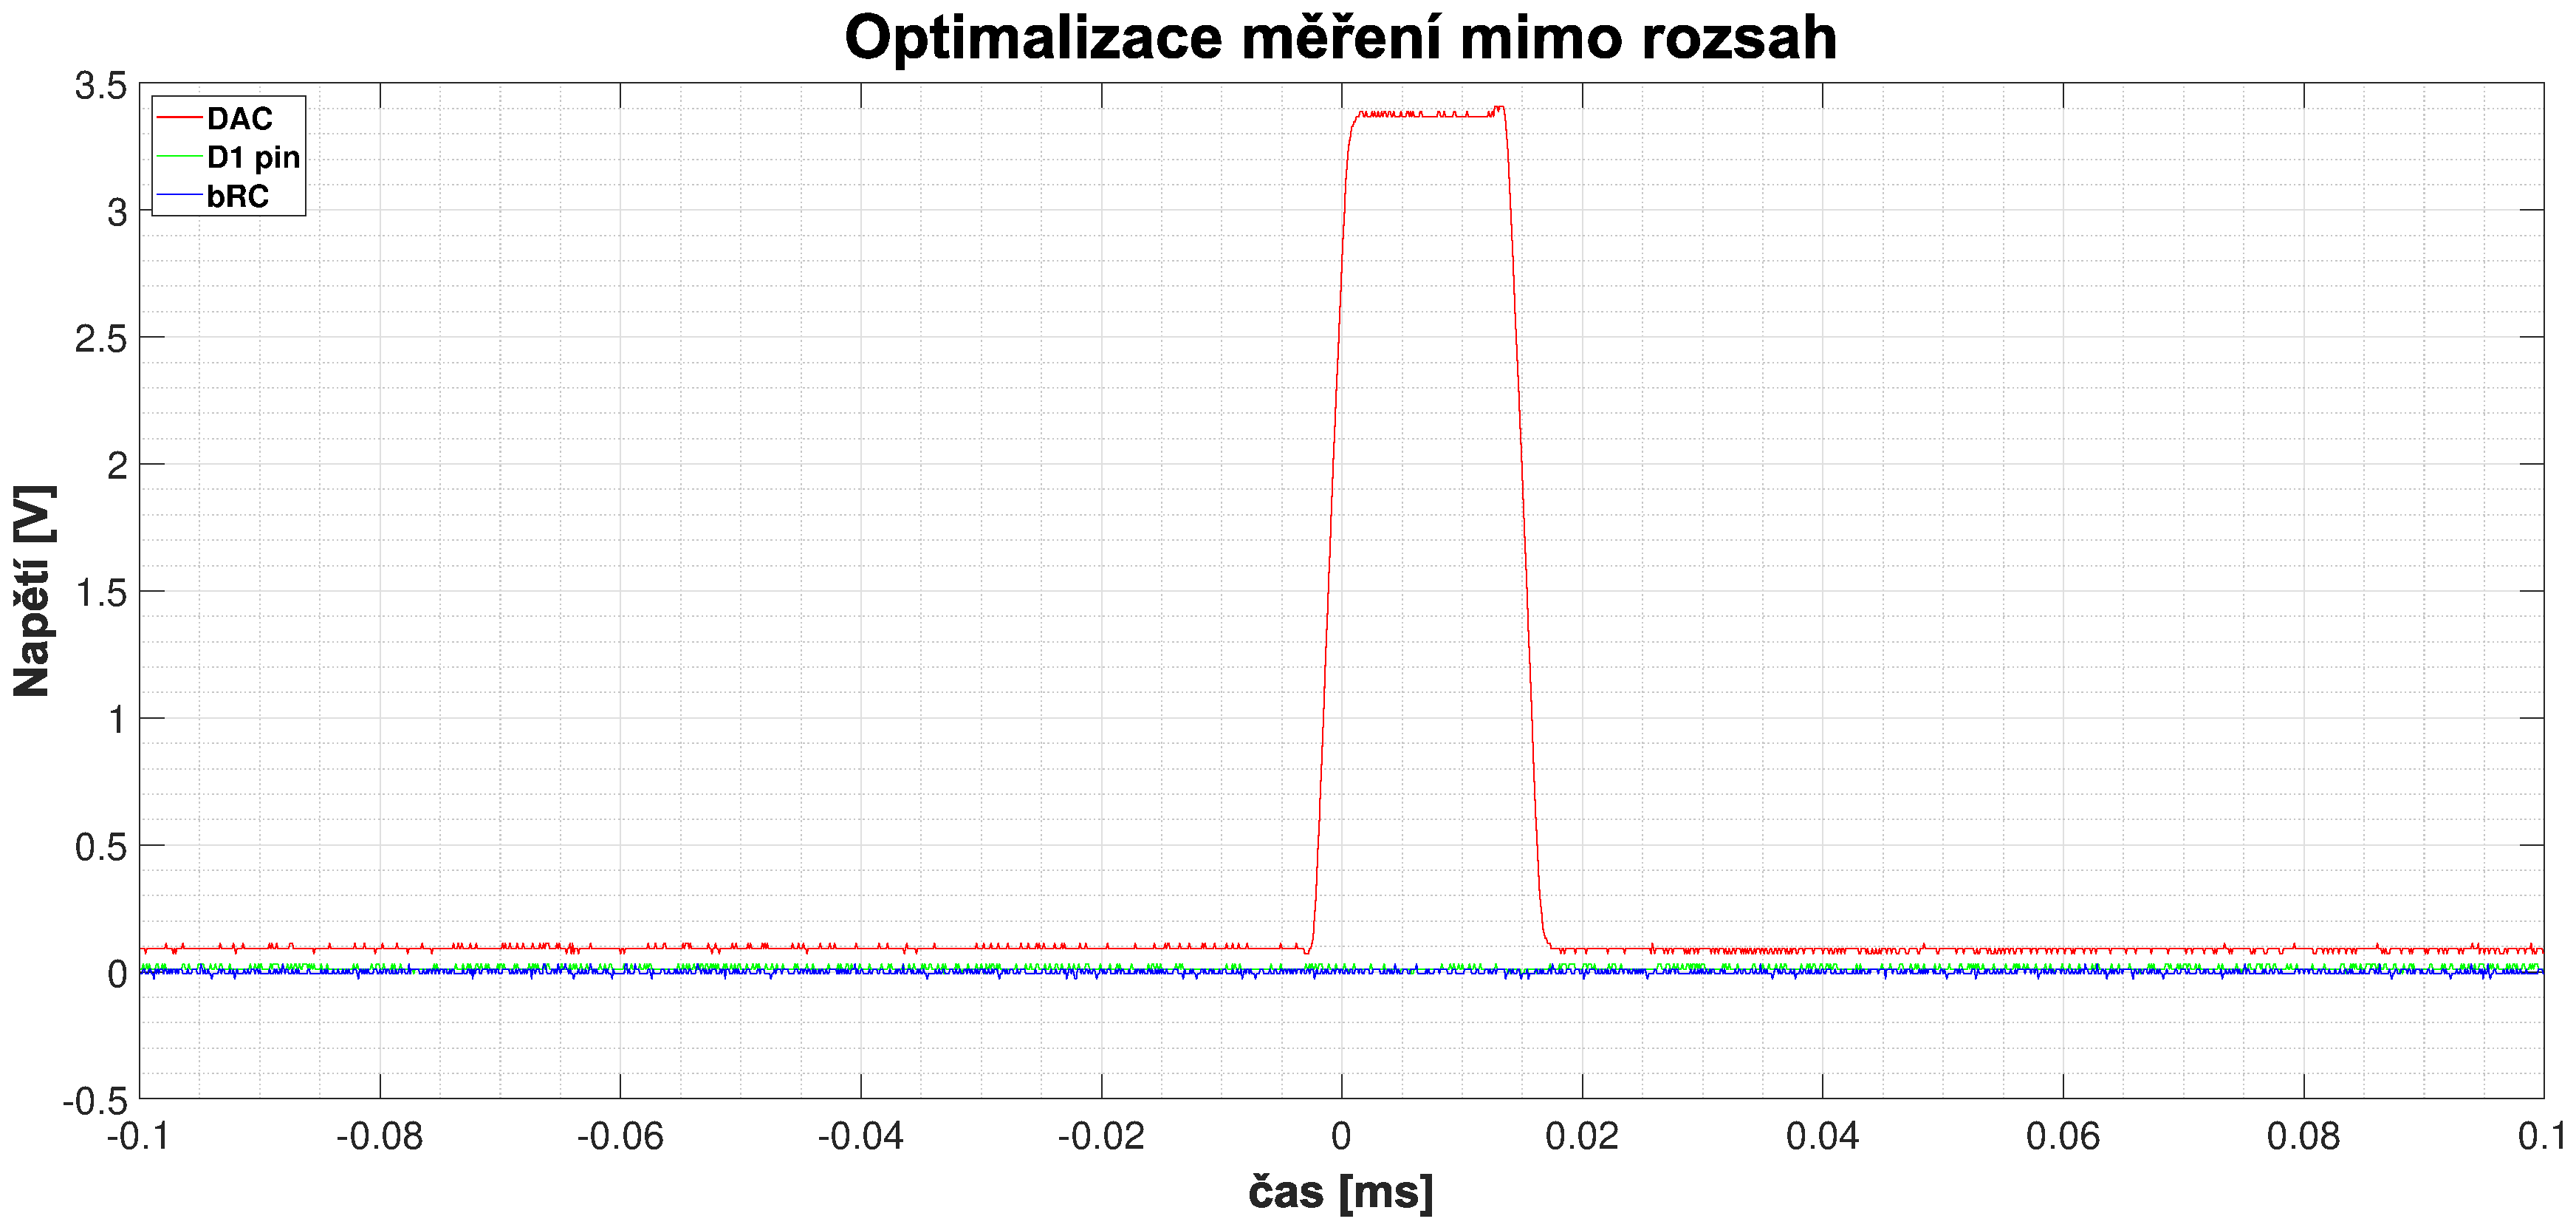
\includegraphics[width = 0.9\textwidth]{obrazky/matlab_generated/pin_out_of_range_opt.eps}
    \caption{Časové průběhy napětí - měření nízkého napětí na bRC pinu optimalizace}
    \label{fig: bRC pin voltage measurement low Voltage opt}
\end{figure}


Vzhledem k charakteru propojení bRC pinů, kde je většina pinů buď propojena tvrdým zkratem (napětí na bRC pinu blízké 3V) nebo rozpojená (napětí na pinu blízké 0V),
vzniká potřeba zkrátit čas měření napětí mimo rozsah D/A převodníku. Z tohoto důvodu je před začátkem měření nejrve změřena logická hodnota výstupu multiplexeru (D1 pin) při
nejnižší a nejvyšší napěťové hodnotě D/A převodníku. Pokud je výstup multiplexeru v obou případech stejný, tak se předpokládá, že je hodnota nižší než dolní mez D/A převodníku
a příkaz vrátí hodnotu -1. Při reálném provozu, tak nemůže nastat situace z obr. \ref{fig: bRC pin voltage measurement low Voltage}.
Měření pak probíhá podle obr. \ref{fig: bRC pin voltage measurement low Voltage opt}. Optimalizované měření pak v případě, že je měřená hodnota mimo rozsah
,trvá pouze přibližně 0.02\,ms nezávisle na použitých konfigurací.\\

Další konfigurace, které lze využít jsou DAC\_RAMP\_MAX\_VALUE\linebreak a DAC\_RAMP\_MIN\_VALUE,
které určují dolní a horní mez rampy D/A převodníku. Tímto lze zkrátit čas měření za cenu nižšího rozsahu.
Zároveň je na tyto mezní hodnoty aplikována stejná metoda jako je popsána v předhozím odstavci. Nicméně nyní dolní mez D/A převodníku nepředstavuje hardwarovou dolní mez měření,
nýbrž mez nastavenou příkazem DAC\_RAMP\_MIN\_VALUE. V případě využívání DAC\_RAMP\_MAX\_VALUE může dojít k měření hodnoty napětí mimo tuto horní mez. Protože pro funkčnost měřící karty není
nutné rozlišovat zda měřená hodnota je nad horní nebo pod dolní mezí a v obou případech vrací příkaz hodnotu -1.\\ 

Prozatím  bylo diskutováno pouze měření napětí na jednom pinu.
V případě \linebreak příkazu 80\_IO\_CARD MEASURE VOLTAGE ALL jsou změřena napětí na všech bRC pinech současně během jedné rampy
D/A převodníku (Obr. \ref{fig: bRC pin voltage measurement allpins}).

\begin{figure}[ht!]
    \centering
    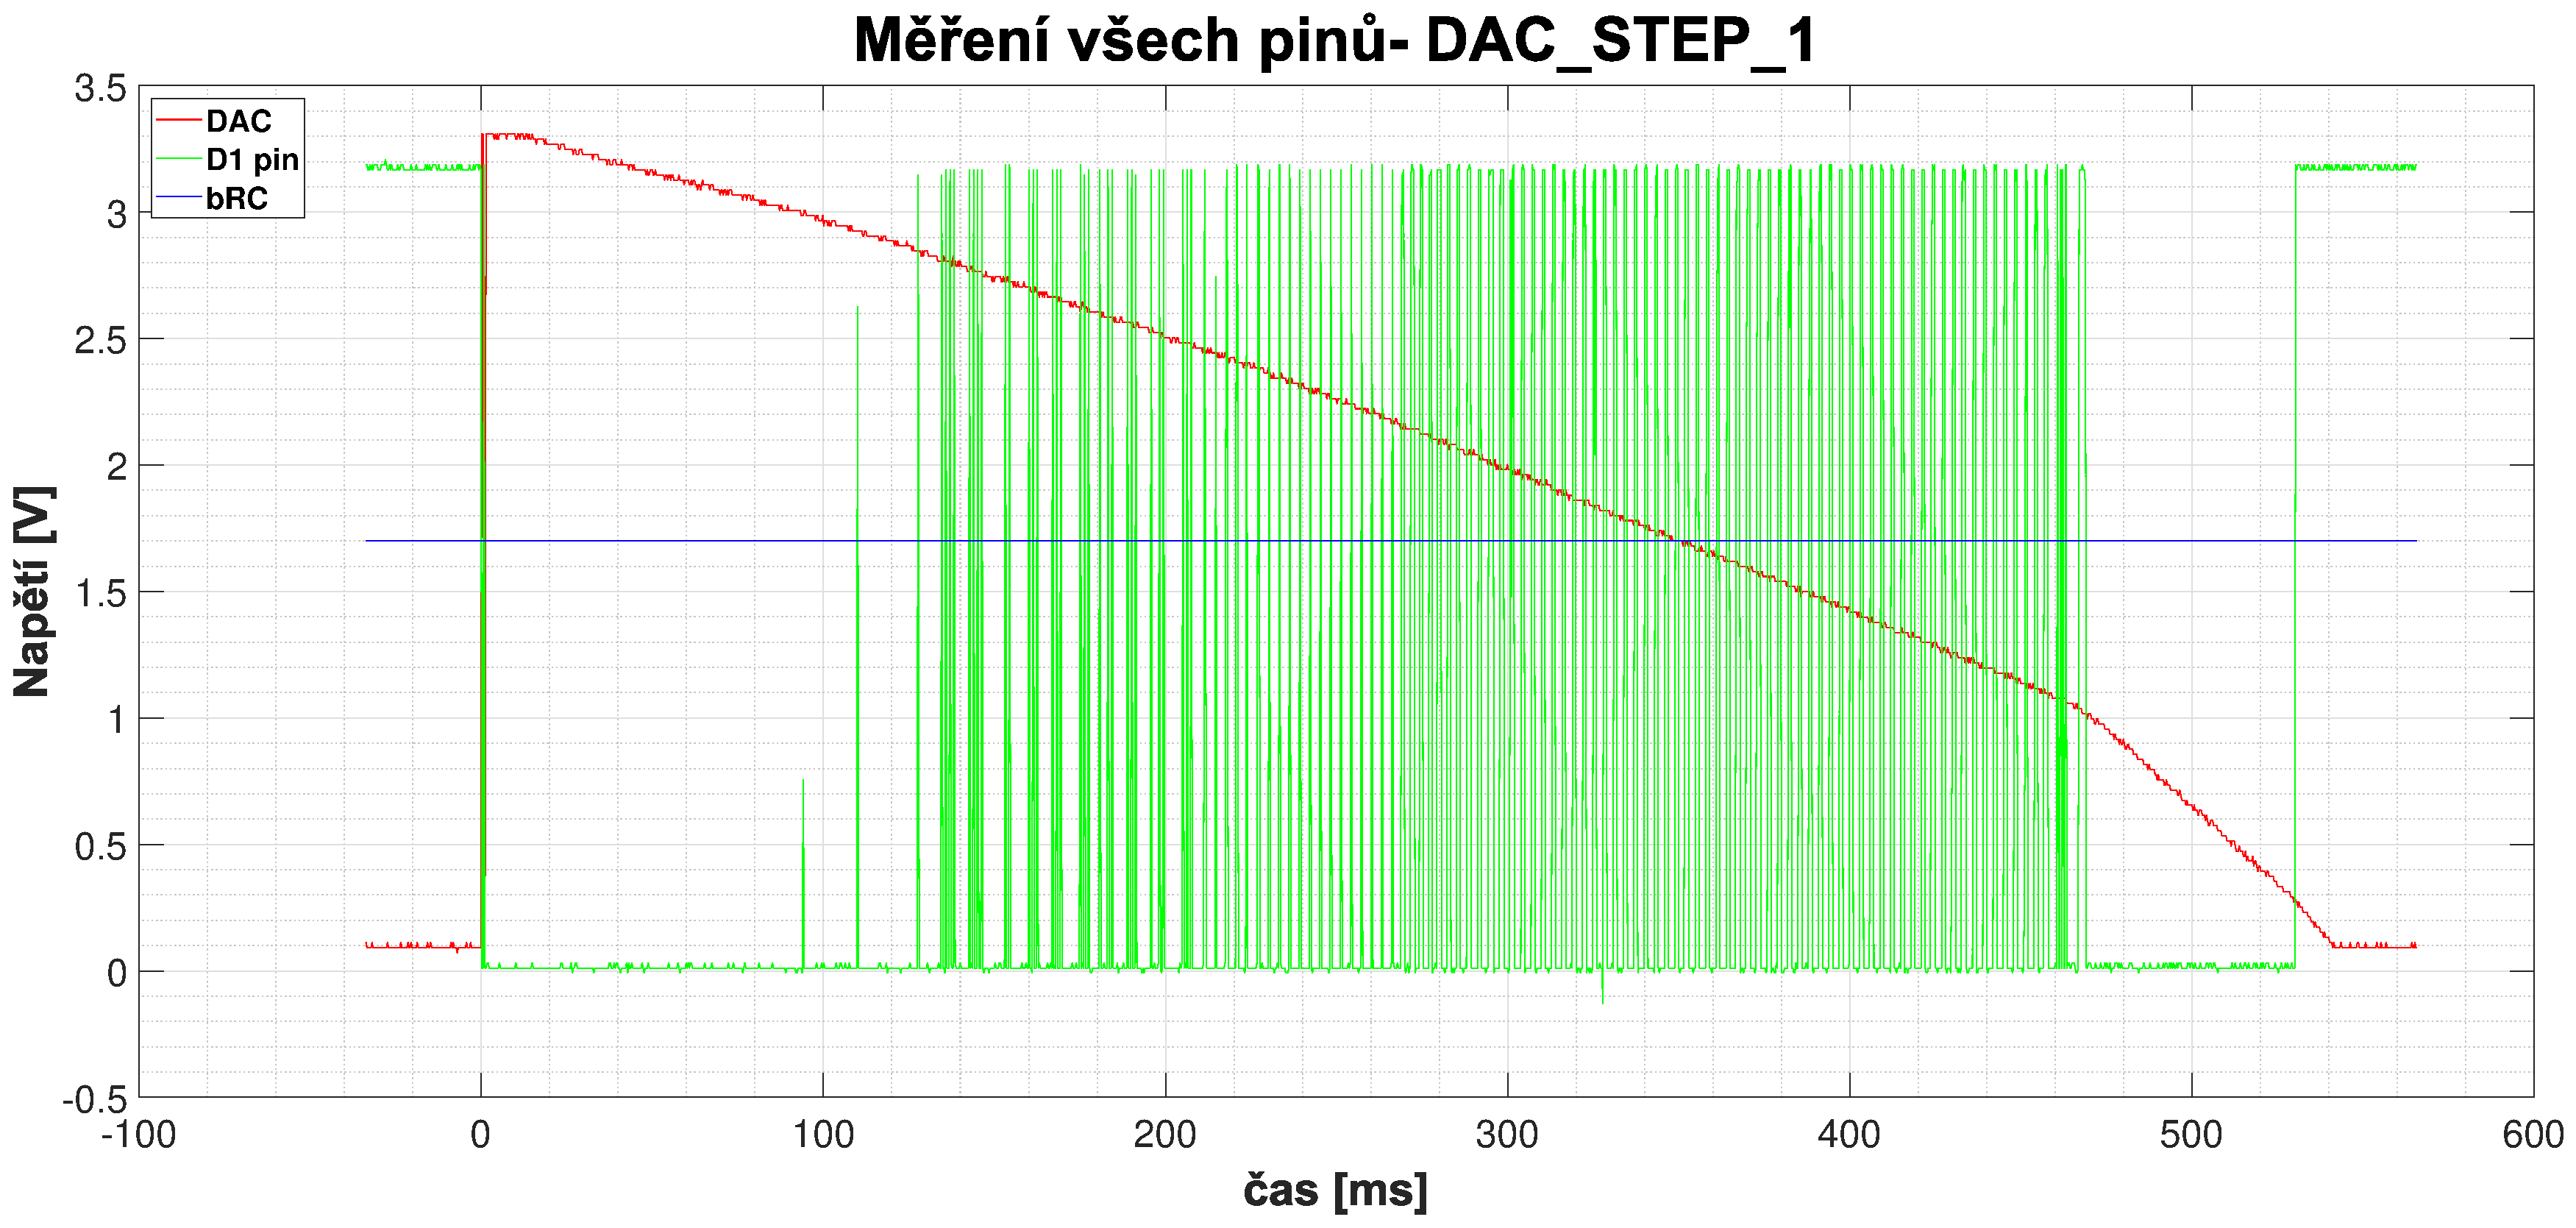
\includegraphics[width = 0.9\textwidth]{obrazky/matlab_generated/all_pins.eps}
    \caption{Časové průběhy napětí - měření napětí na všech pinech současně}
    \label{fig: bRC pin voltage measurement allpins}
\end{figure}

Měření všech pinů probíhá obdobně jako u měření jednotlivých pinů. Nejprve se u všech pinů zkontroluje, zda je měřené napětí v mezích.
Následuje D/A rampa, kde se při každém kroku kontroluje u každého pinu, zda nedošlo k překlopení komparátoru. Pokud dojde k překlopení komparátoru,
tak se uloží aktuální hodnota D/A převodníku do paměti mikrokontroléru. Pokud je pro daný pin již v paměti uložená nějaká hodnota, tak při dalším
kroku D/A rampy již nedochází ke kontrole překlopení komparátoru. To je patrné z obr. \ref{fig: bRC pin voltage measurement allpins}, kde není rampa
D/A převodníku lineární a postupně se měření urychluje s počtem již změřených pinů.\\ 

Zelený průběh napětí na D1 pinu vypadá takto, protože se jedná o výstup multiplexeru. Multiplexery jsou řízeny pomocí společné adresace, takže
se v průběhu měření ,opakovaně a nechtěně, přepíná i výstup již změřeného pinu. Teoreticky by se dalo předpokládat, že takováto aktivita na všech
výstupních pinech multiplexerů bude způsobovat rušení, nicméně při dosavadním měření se tato skutečnost nijak výrazně neprojevila a tak je ignorována.
Případně by rušení šlo do jisté míry omezit správnou posloupností měření pinů.

\subsubsection{MEASURE ADC}
Tento příkaz slouží k změření aktuální hodnoty A/D převodníku. Příkaz vrací hodnotu již přepočtenou na napětí, toto napětí je vztaženo k referenčnímu napětí,
které lze nastavit příkazem 80\_IO\_CARD SET CONFIGURATION VOLTAGE\_REFERENCE

\begin{itemize}[leftmargin=*]
    \item \textbf{Obecný tvar:} 80\_IO\_CARD MEASURE ADC
    \item \textbf{Příklad:}\\
    -> 80\_IO\_CARD MEASURE ADC\\
    <- OK;ADC, value:3.004\\
    \item \textbf{Interpretace odpovědi:} Odpověď obsahuje změřenou hodnotu A/D převodníku vztaženou k referenčnímu napětí.
\end{itemize}